\chapter{Supresión del ruido por \textit{speckle} en imágenes de OCT}
\label{chapter:supresion_ruido_en_oct}

Uno de los principales problemas que tienen las imágenes provenientes de OCT, es que en la mayor parte de los casos se encuentran afectadas por la presencia de ruido de \textit{speckle}. El objetivo de este capítulo es proponer un método de filtrado que preserve las estructuras que se miden con OCT, pero que permita mitigar los efectos del ruido y faciliten la comprensión de la información que poseen las imágenes. Para tal fin, se propone una modificación y extensión de un algoritmo conocido como \textit{non-local means}, considerando las características de la información disponible en OCT. 

El propósito de este capítulo es dar las bases fundamentales para comprender la naturaleza del filtrado propuesto y relacionarlo con los resultados obtenidos. En ese orden de ideas, este capítulo se encuentra dividido en cinco secciones, en donde se analizarán los siguientes aspectos: la Sección~\ref{sec:principios_estadistica_speckle} corresponde a las bases de la estadística de \textit{speckle} de primer orden; la Sección~\ref{sec:estado_arte_filt_speckle} presenta el estado del arte del filtrado de ruido por \speckle en imágenes de OCT; la Sección~\ref{sec:caracteristicas_speckle} discute las causas de la aparición de \speckle en el caso de OCT, fundamento con el que será posible entender la técnica de filtrado que se quiere implementar, y que se discute en la Sección~\ref{sec:from_SAR_to_OCT}. En la última Sección~\ref{sec:resultado_filtrado} se mostrará un análisis de los resultados obtenidos con el filtrado propuesto, y se analizarán algunas aplicaciones en donde se ha probado .

\section{Principios básicos de la estadísticas de \textit{speckle}}
\label{sec:principios_estadistica_speckle}

El \textit{speckle} fue descubierto durante las primeras pruebas realizadas con láseres, en donde se apreciaba la formación de un patrón granulado cuando el haz de luz se reflejaba en superficies tales como las paredes del laboratorio. A partir de estas observaciones, se explicaría que el \speckle surge cuando luz coherente se refleja en una superficie cuya rugosidad se encuentra en la escala de la longitud de onda, o bien, cuando la luz se propaga por un medio con variaciones aleatorias en el índice de refracción \cite{Goodman2010,Dainty1975}. El patrón obtenido bajo estas condiciones posee un alto contraste, con estructuras granulares finas y distribuido en el espacio de una manera relativamente uniforme. La formación de patrones de \speckle es un fenómeno aleatorio, en el que no es posible describir con exactitud en qué lugares aparecerá una estructura brillante u oscura, esto se debe a que la mayor parte de los materiales poseen una rugosidad aleatoria en la escala micro, y su comportamiento no puede ser descrito de manera determinista, sino que debe tratarse mediante funciones de probabilidad que describen las características del campo de \textit{speckle}. Las variaciones aleatorias que son inducidas en el haz para formar patrones de \textit{speckle} en general son complejas, por ende, poseen una amplitud y una fase que representan una magnitud y una dirección aleatoria respectivamente \cite{Goodman1976}. La superposición de las amplitudes y fases aleatorias de todos los puntos luego de la reflexión en la superficie, dan lugar a la formación del patrón de \textit{speckle}. Esta suma produce que la amplitud y la fase sean aleatorias, y de acuerdo a la diferencia de fase que haya entre los puntos en la superficie o las contribuciones elementales se producirá interferencia constructiva o destructiva, por lo tanto el \speckle tendrá una apariencia de puntos brillantes u oscuros respectivamente.


%El \textit{speckle} fue descubierto durante las primeras pruebas realizadas con láseres, en donde se apreciaba la formación de un patrón granulado cuando el haz de luz se reflejaba en superficies tales como las paredes del laboratorio. A partir de estas observaciones, se explicaría que el \speckle surge cuando luz coherente se refleja en una superficie cuya rugosidad se encuentra en la escala de la longitud de onda, o bien, cuando la luz se propaga por un medio con variaciones aleatorias en el índice de refracción \cite{Goodman2010,Dainty1975}. El patrón obtenido bajo estas condiciones posee un alto contraste, con estructuras granulares finas y distribuido en el espacio de una manera relativamente uniforme. Dado que la rugosidad que poseen la mayor parte de los materiales es aleatoria, el patrón de \speckle obtenido sigue también una forma aleatoria, por lo que sus características deben describirse como funciones de probabilidad que relacionan las propiedades del campo de \speckle. Las variaciones aleatorias que son inducidas en el haz para los patrones de \speckle son, en general, complejas, por lo tanto, poseen una amplitud y una fase, representando una magnitud y una dirección aleatoria respectivamente \cite{Goodman1976}. El patrón de \speckle formado posee entonces la superposición de todas las contribuciones elementales al campo luego de la reflexión en la superficie, esta superposición produce que la amplitud y la fase sean aleatorias, y de acuerdo a la diferencia de fase que haya entre las contribuciones elementales, se formará dará interferencia constructiva o destructiva y como consecuencia de esto, el patrón de \speckle tiene una apariencia de puntos brillantes y oscuros distribuidos en el espacio.

%La superposición o suma de todas las contribuciones del campo complejo luego de reflejarse en la superficie producen un patrón de interferencia constructiva o destructiva, apareciendo como puntos brillantes u oscuros. 


%El \textit{speckle} surge cuando luz coherente es reflejada por una superficie cuya rugosidad se encuentra en la escala de la longitud de onda, o bien cuando la luz se propaga por un medio con variaciones aleatorias del índice de refracción\cite{Goodman2010,Dainty1975}. El patrón que se obtiene bajo estas condiciones posee un alto contraste con estructuras finas granulares y distribuido de una forma relativamente uniforme. Las primeras observaciones de patrones de \speckle se dieron con la aparición de los primeros láseres, ya que luego de esto interactuar con superficies que en la escala macro parecen lisas, pero que desde una perspectiva microscópica son rugosas. Debido a que la rugosidad que poseen la mayor parte de los materiales es aleatoria, el patrón de \speckle obtenido sigue también una forma aleatoria. Las variaciones que son introducidas en la luz, pueden ser complejas, con una amplitud y una fase que representan una longitud y una dirección aleatoria respectivamente. La superposición o suma de todas las contribuciones del campo complejo luego de reflejarse en la superficie producen un patrón de interferencia constructiva o destructiva, apareciendo como puntos brillantes u oscuros. 

Debido a que no se conocen detalles sobre la estructura microscópica de la superficie, es más fácil analizar las características de los patrones de \speckle de manera estadística \cite{Dainty1975}, asumiendo que sus propiedades en la escala microscópica difieren. Si $\boldsymbol{A}(x,y,t)$ es una señal compleja en el patrón de \textit{speckle} en un punto $(x,y)$ en un instante $t$, ésta puede representarse como

%Debido a que no se conocen detalles sobre la estructura microscópica de la superficie, es más fácil analizar las características de los patrones de \speckle de manera estadística \cite{Dainty1975}, con esto, se asume que las propiedades en la escala macro de un objeto son iguales, pero difieren en la escala micro. Una señal compleja $\boldsymbol{A}(x,y,t)$ en un punto $(x,y)$ en un instante $t$, puede representarse como,

\begin{equation}
\boldsymbol{A}(x,y,t) = A(x,y,t)e^{i\theta(x,y,t)},
\end{equation}

\noindent donde $A(x,y,t)$ es la amplitud, $\theta(x,y,t)$ la fase y $(x,y,t)$ la dependencia espacial y temporal de dicha señal. El patrón de \speckle aparece cuando cada punto se encuentra descrito a través de la superposición de una gran cantidad de contribuciones elementales complejas $\boldsymbol{a_n}(x,y,t)$ con fases aleatorias provenientes de $N$ puntos diferentes y producidas por centros dispersores, de manera que el campo de \speckle obtenido corresponde a 

\begin{align}
\boldsymbol{A}(x,y,t) &= A(x,y,t)e^{i\theta(x,y,t)} \notag\\ 
&= \frac{1}{\sqrt{N}}\sum_{n=1}^{N} \boldsymbol{a_n}(x,y,t) \notag\\
&= \frac{1}{\sqrt{N}}\sum_{n=1}^{N} a_n(x,y,t) e^{i\phi_n(x,y,t)},
\end{align}

%\noindent donde $\boldsymbol{a_n}(x,y,t)$ es el n-enésimo punto contribuyente al campo, con amplitud $a_n(x,y,t)$ y fase $\phi_n(x,y,t)$. La estadística de \speckle busca describir el campo complejo $\boldsymbol{A(x,y,t)}$ a partir de cálculos estadísticos de la superposición de las contribuciones elementales, para describir así la probabilidad de que un punto en el espacio y tiempo posea una amplitud $A(x,y,t)$ y una fase $\theta(x,y,t)$. En los últimos dos parámetros se centrará el análisis, en base a las contribuciones elementales $a_n(x,y,t)$ y $\phi(x,y,t)$, por lo tanto se asumirá que \cite{Goodman2010}: (1) la amplitud $a_n$ y la fase $\phi_n$ de las contribuciones elementales, son estadísticamente independientes de $a_m$ y $\phi_m$ cuando $n\neq m$, es decir, la amplitud y la fase de las contribuciones elementales no aportan información sobre la amplitud y fase de otra contribución elemental diferente a sí misma; (2) para cualquier $n$ la amplitud $a_n$ y la fase $\phi_n$ son estadísticamente independientes, por lo tanto, conocer la amplitud $a_n$ no aporta información sobre la fase $\phi_n$ y viceversa; (3) las fases de las contribuciones elementales $\phi_n$ se encuentran distribuidas en el intervalo $(-\pi, \pi)$, esto es que la fase tiene la misma probabilidad de adquirir cualquier valor de fase en un rango de $2\pi$. 

\noindent donde $\boldsymbol{a_n}(x,y,t)$ es el n-enésimo punto contribuyente al campo, con amplitud $a_n(x,y,t)$ y fase $\phi_n(x,y,t)$. El campo complejo $\boldsymbol{A}(x,y,t)$ se describe a partir de la \textit{estadística de speckle}, en donde cálculos estadísticos de la superposición de las contribuciones elementales describen la probabilidad de que un punto en el espacio y tiempo, posea una amplitud $A(x,y,t)$ y una fase $\theta(x,y,t)$. En estos parámetros se centrará el análisis, basándose en las contribuciones elementales $a_n(x,y,t)$ y $\phi(x,y,t)$, para ello se asumirá que \cite{Goodman2010}: (1) la amplitud $a_n$ y la fase $\phi_n$ de las contribuciones elementales son estadísticamente independientes de $a_m$ y $\phi_m$ cuando $n\neq m$, es decir, la amplitud y la fase de las contribuciones elementales no aportan información sobre la amplitud y la fase de otra contribución elemental diferente a sí misma; (2) para cualquier $n$ la amplitud $a_n$ y la fase $\phi_n$ son estadísticamente independientes, por lo tanto, conocer la amplitud $a_n$ no aporta información sobre la fase $\phi_n$ y viceversa; (3) las fases de las contribuciones elementales $\phi_n$ se encuentran distribuidas en el intervalo $(-\pi, \pi)$, por lo tanto, fase tiene la misma probabilidad de adquirir cualquier valor en un rango de $2\pi$.

La función de densidad de probabilidad conjunta $p_{A,\theta}(A,\theta)$ para la amplitud y la fase del campo resultante de la superposición de contribuciones elementales, obedece a la ecuación \cite{Goodman2010}

\begin{equation}
\label{eq:p_a_theta}
p_{A,\theta}(A,\theta) = \frac{A}{2\pi\sigma^2}\exp\left(-\frac{A^2}{2\sigma^2}\right),
\end{equation}

\noindent donde $\sigma$ es la varianza de la amplitud, esto se cumple para el rango $(A\geq0)$ y $(-\pi\leq\theta<\pi)$. A partir de la función de densidad de probabilidad conjunta se puede encontrar la estadística de $A$ y $\theta$ de manera individual, en el primer caso integrando la Eq.~\ref{eq:p_a_theta} con respecto a $\theta$, mientras que en el segundo caso integrando con respecto a la amplitud $A$. La función de densidad de probabilidad para la amplitud $p_A(A)$ se calcula con la Eq.~\ref{eq:p_a_theta} e integrando respecto a $\theta$ en el intervalo acotado sigue que

\begin{equation}
\label{eq:prop_a}
p_A(A) = \int_{-\pi}^{\pi}p_{A,\theta}(A,\theta) d\theta = \frac{A}{\sigma^2}\exp\left(-\frac{A}{2\sigma^2}\right),
\end{equation}

\noindent la cual corresponde a una función de Rayleigh, esto concluye que la amplitud de una campo de \speckle sigue una función de densidad de probabilidad del tipo Rayleigh. Si bien la Eq.~\ref{eq:prop_a} describe la probabilidad de obtener algún valor de amplitud específico, los sensores digitales solamente pueden registrar la intensidad $I$ del patrón, que se define como el módulo cuadrado de la amplitud $I = \lvert \boldsymbol{A}\rvert^2$. 

Conocer la probabilidad de obtener algún valor de intensidad es de alta importancia, ya que describe los valores que se registrarán en el detector. La función de densidad de probabilidad en el caso de la intensidad se obtiene entonces como

%La intensidad $I$, que corresponde al módulo cuadrado de la amplitud es de alta importancia ya que es la medición que puede hacerse del campo, y se define como

%\begin{equation}
%\label{eq:I}
%I = \lvert \boldsymbol{A}\rvert^2.
%\end{equation}

%La función de densidad de probabilidad para la intensidad en el patrón de \speckle se encuentra empleando la Eq.~\ref{eq:I} y la Eq.~\ref{eq:prop_a}, esto es

\begin{align}
\label{eq:p_I}
p_I(I) &= p_A(A) \times p_A^{\ast}(A) = \lvert p_A(A)\rvert ^2, \notag\\
&= \frac{1}{2\pi\sigma^2}\exp\left(-\frac{I}{2\sigma^2}\right)\notag\\
&= \frac{1}{\bar{I}}\exp\left(-\frac{I}{\bar{I}}\right),
\end{align}

%\noindent donde $\bar{I}$ es el valor esperado de la intensidad, esto se cumple para $(I\geq0)$. La distribución correspondiente a la Eq.~\ref{eq:p_I} es una función de densidad de probabilidad exponencial negativa, a los patrones de \speckle que siguen esta distribución de intensidad, se les conoce como \textit{speckle completamente desarrollado}, y cumplen que la varianza de la intensidad, es igual a su valor esperado,

\noindent donde $\bar{I}$ es el valor esperado de la intensidad, esto se cumple para $(I\geq0)$. La distribución correspondiente a la Eq.~\ref{eq:p_I} es una función de densidad de probabilidad exponencial negativa, e indica que es más probable obtener regiones oscuras que brillantes en el patrón de \textit{speckle} debido a que la probabilidad de obtener una intensidad alta decrece exponencialmente. A los patrones de \speckle que siguen este tipo de distribución de intensidad, se les conoce como \textit{speckle completamente desarrollado}, y cumplen que la varianza de la intensidad, es igual a su valor esperado,
\begin{align}
\sigma_I^2 &= \bar{I}^2 \notag\\
\sigma_I & = \bar{I}.
\end{align}
A partir de esto, en el caso del \speckle completamente desarrollado \cite{Goodman1976}, la relación señal ruido definida en la Sección~\ref{subsec:SNR}, corresponde a $SNR = \bar{I}/\sigma_I = 1$, como consecuencia de esto, el ruido causado por \speckle tiene fluctuaciones del orden de la señal y degrada fuertemente la calidad de las imágenes que se capturan cuando éste se presenta. Finalmente, la función de densidad de probabilidad para el caso de la fase $p_{\theta}(\theta)$, se puede hallar integrando la Eq.~\ref{eq:p_a_theta} con respecto a $A$, esto es

\begin{equation}
p_\theta (\theta) = \int_{0}^{\infty} \frac{A}{2\pi\sigma^2}\exp\left(-\frac{A^2}{2\sigma^2}\right)dA = \frac{1}{2\pi},
\end{equation}

\noindent es decir que todos los puntos tienen la misma probabilidad de tener un valor de fase distribuido en un intervalo de $2\pi$.

%FALTA UN PÁRRAFO PARA UNIR ESTO CON LA PARTE DEL ESTADO DEL ARTE, PROBABLEMENTE SEA SUFUCIENTE MENCIONAR DÓNDE APARECE SPECKLE

El \speckle aparece en técnicas de imagen coherente y por lo general, se manifiesta como ruido en las imágenes. Algunas técnicas de imagen en donde aparece el ruido por \speckle son: imágenes de radares de apertura sintética (SAR: \textit{synthetic-aperture radar}) \cite{Deledalle2015}, imágenes de ultrasonido \cite{Kalaivani2009}, tomografías computacionales (CT: \textit{computed tomography}) \cite{Sidky2008}, imágenes por resonancia mágnetica (MRI: \textit{magnetic resonance imaging}) \cite{Pizurica2006}  e imágenes de OCT \cite{Schmitt1999}. El ruido por \speckle reduce el contraste de estructuras finas y dificulta la interpretación de información relevante en las técnicas mencionadas anteriormente, sin embargo, su aparición es inherente a las propiedades de los sistemas con los cuales se capturan las imágenes. En cada una de las categorías de imagen mencionadas anteriormente, existen diversas técnicas que permiten reducir el impacto del ruido por \speckle mediante modificaciones en el método de captura de datos \cite{Lee1994} o a  través técnicas que son realizadas por posprocesamiento \cite{Lu2011}. A continuación, se detallará el desarrollo que han tenido algunas técnicas de posprocesamiento en el caso de OCT.

\section{Estado del arte del filtrado de \speckle en OCT}
\label{sec:estado_arte_filt_speckle}

Como en los casos de imagen coherente, el \speckle aparece en OCT de dos maneras: como señal portadora de información y a la vez como degradador de la señal en forma de ruido \cite{Schmitt1999}, sin embargo, la discusión de este aspecto se dejará para la Sección~\ref{sec:caracteristicas_speckle}. Los algoritmos desarrollados para eliminar el ruido por \speckle en OCT pueden dividirse en tres grandes categorías: descomposición en transformaciones \cite{Adler2004, Mayer2012}, representaciones dispersas (\textit{sparse}) \cite{Fang2012} y filtros en el dominio espacial \cite{Yu2016}. En el caso de las transformadas se encuentran algoritmos conocidos como \textit{wavelet} \cite{Adler2004, Mayer2012} y \textit{curvelet} \cite{Jian2009,Xu2013} en donde el filtrado se realiza a través del cálculo de coeficientes asociados con la imagen, aquellos coeficientes que provienen de los bordes de la imagen se agrupan espacialmente, mientras que aquellos provenientes de los patrones de \speckle no. Los coeficientes correspondientes al ruido y a la imagen pueden diferenciarse por medio de un umbral, lo que permite reducir la discontinuidades causadas por el \textit{speckle} en la imagen. Éstas técnicas tienen la desventaja de ser poco sensibles ante estructuras finas y pueden producir artefactos en las imágenes filtradas cerca a los bordes.

Las representaciones \textit{sparse} se encuentran relacionadas con el concepto de \textit{compress sensing}, y en general, emplean una porción del total de datos para remover el ruido de manera efectiva en toda la imagen \cite{Xu2012,Fang2012,Fang2013,Fang2015}. El filtrado mediante representaciones \textit{sparse}, conocido como \textit{multiscale sparsity-based tomographic denoising} (MSBTD) \cite{Fang2012} requiere la captura de un patrón de datos especial, en donde la velocidad de captura es muy baja, y por tanto, hay una alta relación señal-ruido. Con base en ese patrón especial, se crean diccionarios contra los cuales se comparan y filtran las imágenes capturadas a una mayor velocidad y una relación señal ruido menor, asumiendo que los vecinos cercanos a un punto poseen una textura y un patrón de ruido similar. Extensiones al MSBTD han sido propuestas \cite{Fang2013, Fang2015}, en donde los diccionarios se crean a partir de datos previamente adquiridos y mejoran el desempeño del filtrado, no obstante, esta mejora trae consigo un incremento significativo en el tiempo de procesamiento de los datos.

Los filtros en el dominio espacial pueden categorizarse en dos grupos principales, locales y no locales. Los algoritmos locales, tales como la divergencia de regularización generalizada (GDR: \textit{generalized divergence regularization}) \cite{Cheng2012}, tienen bajos tiempo de computo, pero la desventaja de no funcionar muy bien cuando la correlación entre píxeles cercanos se ha perdido por culpa del ruido o cuando la relación señal ruido es baja. En los métodos no locales, como el promedio no local (\textit{NL-Means}: \textit{non-local means}) \cite{Baudes2005, Deledalle2009} emplean una pequeña región alrededor de cada pixel para realizar el filtrado, en lugar de considerar cada pixel de manera independiente. \nlmeans ha sido altamente atractivo para el filtrado de ruido gaussiano y se ha extendido hasta el caso de ruido multiplicativo o de \textit{speckle}. Recientemente, \nlmeans se implementó en OCT por Yu \etal \cite{Yu2016}, y su desempeño ha sido comparable con otros algoritmos de filtrado empleados en OCT hasta la fecha.

%\section{Estado del arte del filtrado de \speckle en algunas técnicas de imagen coherente}
%El ruido por \speckle aparece en técnicas de imagen coherente, como lo son imágenes de radares de apertura sintética (SAR: \textit{synthetic-aperture radar}), imágenes de ultrasonido, tomografías computacionales (CT: \textit{computed tomography}), imágenes por resonancia mágnetica (MRI: \textit{magnetic resonance imaging}) e imágenes de OCT, se encuentran entre las técnicas de imagen que más sufren de este tipo de ruido. En general, en cada una de estas categorías, diferentes alternativas que permiten reducir el impacto del \speckle, el cual reduce el contraste de estructuras finas y dificulta la interpretación de la información, han sido desarolladas. 

%El ruido por \speckle aparece en técnicas de imagen coherente, como lo son imágenes de radares de apertura sintética (SAR: \textit{synthetic-aperture radar}) \cite{Deledalle2015}, imágenes de ultrasonido \cite{Kalaivani2009}, tomografías computacionales (CT: \textit{computed tomography}) \cite{Sidky2008}, imágenes por resonancia mágnetica (MRI: \textit{magnetic resonance imaging}) \cite{Pizurica2006}  e imágenes de OCT \cite{Schmitt1999}. El ruido por \speckle, en general, reduce el contraste de estructuras finas y dificulta la interpretación de información relevante en las técnicas mencionadas anteriormente, sin embargo, su aparición es inherente a las propiedades de los sistemas con los cuales se capturan las imágenes. En cada una de las categorías de imagen mencionadas anteriormente existen diversas técnicas que permiten reducir el impacto del ruido por \speckle, mediante modificaciones en el método de captura de datos a través del promedio de múltiples imágenes, proceso conocido como \textit{multilooking} \cite{Lee1994}; hasta técncias que son realizadas por posprocesamiento \cite{Lu2011}.

%El filtrado de ruido es un área ampliamente investigada, ya que la creación de dispositivos de bajo costo y fácil acceso en diferentes disciplinas, acarrea dificultades que deben solucionarme mediante procedimientocada vez más precisos. Aunque cada área de la ciencia implementa métodos de filtrado acorde a las características de las imágenes adquiridas, se pueden agrupar las técnicas de las cuales estos provienen en algunas categorías, para el caso del ruido

%En el caso de OCT, 
%Entre las técnicas más comunes para la reducción de ruido por \speckle se ecuentra el \multilooking, el cual consiste en promediar una cantidad $N$ de imágenes de la misma escena, cuyas realizaciones de \speckle sean diferentes. Este tipo de filtrado, reduce el ruido en un factor de $\sqrt{N}$, pero tiene la desventaja de incrementar altamente el tiempo de captura de las imágenes. Una forma en la que se puede realizar el proceso de \multilooking sin que se requeira capturar múltiples imágenes, es mediante una reducción del espectro en el cual se capturan las imágenes, aunque este procedimiento tiene la desventaja de reducir altamente la resolución de la imagen. Sin embargo, han aparecido otros métodos que realizan procesos similares, pero no reducen la reslución espacial de las imágenes, como lo son: 

%En el caso de OCT, algunas técnicas que se han empleado corresponden a 

%Recientemente, una técnica proveniente de SAR, y conocida como promedio no local (NL-Means: \textit{non-local means}) se ha empleado en OCT. Nuestro objetivo es emplear y mejorar NLMeans para seer implementado en el casod de OCT.

\section{Características del \textit{speckle} en OCT}
\label{sec:caracteristicas_speckle}

Como se mencionó anteriormente, las características del patrón de \speckle que se produce cuando la luz se refleja en una superficie rugosa o al pasar por un medio con variaciones en el índice de refracción depende de las características de dichos medios, muestra de ello es que desplazamientos pequeños de la superficie rugosa varían completamente la forma que posee el patrón de \textit{speckle}. En el caso de OCT, el \speckle es influenciado no sólo por las propiedades de los medios, sino que depende también de la coherencia temporal de la fuente, las refracciones y aberraciones que experimenta el haz, así como de la apertura numérica del sistema \cite{Schmitt1999}. En OCT, la señal que se captura proviene de la interferencia producida por un haz de referencia y la señal retroreflejada por la muestra, mientras que el escaneo axial es posible ya que la interferencia se da unicamente en profundidades dentro de la longitud de coherencia. 

La fotocorriente producida en el detector $i_D$, es proporcional al promedio temporal de la suma del haz referencia $E_R$ y el haz objeto $E_s$, reescrito desde la Eq.~\ref{eq:I_1},

\begin{equation}
i_D = \rho \langle\lvert E_R+E_S \rvert^2\rangle
\end{equation}

\noindent donde $\langle \cdot \rangle$ representa el promedio temporal que realiza el detector y $\rho$ es el factor de respuesta del sensor. La señal interferométrica que se mide corresponde entonces a

\begin{equation}
i_D = \rho \langle\lvert E_R\rvert^2 + \lvert E_S \rvert^2 + 2E_R E_S \cos(\phi)\rangle,
\end{equation}

\noindent donde $\phi$ representa la diferencia de camino óptico entre ambos haces ($\phi = 2 k_0 \Delta z$), nótese que la fotocorriente $i_D$ depende de la diferencia de camino óptico entre los brazos, esto es lo que hace que OCT sea sensible a la fase y por tanto al ruido por \textit{speckle}. 

En el caso ideal de un solo reflector ubicado en el brazo objeto y que refleja la totalidad de la luz que recibe, la fotocorriente depende unicamente de la diferencia de camino óptico entre los haces. En el caso de las muestras de OCT, se tiene una alta densidad de centros dispersores en la muestra, lo que produce una modulación en el patrón de interferencia que dependerá de la forma en la que se superpongan las distintas contribuciones de la totalidad de los centros dispersores. La luz que se propaga en la muestra tiene dos principales componentes de aleatoriedad, una de ellas introducida por las múltiples dispersiones que sufre el haz al entrar y salir del tejido; la segunda, es causada por el esparcimiento que sufre al propagarse de ida y regreso. 

La Fig.~\ref{fig:sample_backscattering} ejemplifica el recorrido que sigue la luz al interior de la muestra, inicialmente, un frente de onda incidente llega hasta la muestra, luego se darán múltiples dispersiones y esparcimientos en el camino de entrada hasta llegar a la región focal en donde se obtiene imagen. En el camino de regreso, la luz debe experimentar nuevamente dispersiones y esparcimientos hasta regresar al sistema óptico, en este proceso, el frente de onda ha sufrido una deformación por los retrasos aleatorios que sufre al retornar. Adicionalmente, hay centros dispersores por fuera de la zona focal que pueden reflejar luz en la dirección del detector, al igual que centros dispersores que luego de múltiples esparcimientos regresan luz al sistema óptico. La contribución de estos puntos, es lo que genera que el frente de onda experimente interferencias aleatorias, dando lugar a la aparición de \speckle en las imágenes registradas.

\begin{figure}
\centering
\includegraphics[width=0.4\linewidth]{img/chap3/sample_backscattering}
\caption[Formación del \speckle en OCT.]{El \speckle en OCT se forma a causa de las múltiples propagaciones que debe realizar el haz en la muestra hasta llegar a la región focal, el esparcimiento y la dispersión al ingreso y salida del tejido produce una aleatorización del frente de onda, y por tanto, se da la formación de patrones de \textit{speckle}.}
\label{fig:sample_backscattering}
\end{figure}

Los resultados de la estadística de \speckle obtenidos en imágenes de OCT por Schmitt \etal \cite{Schmitt1999} y por Bashkansky \etal \cite{Bashkansky2000} muestran que los patrones de \speckle que se forman en OCT en el caso de luz polarizada quasimonocromática, son patrones completamente desarrollados, donde la probabilidad de medir un valor de intensidad $p(I)$ en algún punto, obedece una a función de densidad de probabilidad exponencial decreciente,

\begin{equation}
p(I) = \frac{1}{\bar{I}}\exp\left(-\frac{I}{\bar{I}}\right), \notag
\end{equation}

\noindent como se explicó en la Sección~\ref{sec:principios_estadistica_speckle}. Pero en el caso de luz despolarizada, hay una variación en la función de densidad de probabilidad de los patrones obtenidos, esta corresponde a \cite{Bashkansky2000},

\begin{equation}
\label{eq:p_i_oct}
p(I) = \frac{4I}{\bar{I}}^2\exp\left(-2\frac{I}{\bar{I}}\right).
\end{equation}

\noindent En el caso de luz no polarizada, la relación señal ruido tiene también una variación, incrementándose a $SNR=1.4$, esto es un aumento de $0.4$ con respecto al caso de luz polarizada, este hecho es parcialmente soportado por la falta de influencia del estado de polarización en la interferencia aleatoria para formar patrones de \textit{speckle}.

%El problema fundamental que tiene el \speckle en OCT es que cumple una doble función que imposibilita el hecho de eliminarlo completamente. En este sentido, el \speckle se divide en dos categorías: \speckle portador de señal y \speckle degradador de señal \cite{Schmitt1999}. En el mejor de los casos de un sistema de OCT, el \speckle portador de señal proveniente desde la muestra corresponde a una única retroreflexión del campo esparcido por la muestra, esto implica que la luz debe propagarse a través del tejido sin esparcirse ni dispersarse, luego reflejarse solamente en una partícula de la muestra y regresar en la dirección del detector una vez más sin sufrir esparcimiento o dispersión. En la mayor parte de los tejidos, estas condiciones son prácticamente inexistente, y el  \speckle portador de señal se encuentra influenciado por la correlación con el \speckle degradador de señal. Los puntos que generan \speckle degradador se encuentran compuestos por aquellas regiones fuera de la zona focal y sufren esparcimiento múltiples veces, de forma que regresan con una fase aleatoria impuesta por la diferencia de camino óptico.

El problema fundamental que tiene el \speckle en OCT es que cumple una doble función, lo que imposibilita su eliminación completamente. En este sentido, el \speckle se divide en dos categorías: \speckle portador de señal y \speckle degradador de señal \cite{Schmitt1999}. El \speckle portador de señal se origina desde la muestra en la zona focal, y proyecta en promedio, un tamaño proporcional a la muestra medida. El \speckle degradador consiste de pequeños puntos de \speckle creados por la luz que llega a regiones fuera de la zona focal, y luego, es dispersada múltiples veces hasta que retorna al sistema con una diferencia de camino óptico con respecto a los brazos del interferómetro, manifestándose como ruido. 

El tamaño del \speckle puede controlarse a través de variaciones en la apertura numérica del sistema óptico, una apertura numérica menor produce patrones de \speckle relativamente grandes, mientras que una apertura numérica grande genera patrones más finos. Una imagen de la retina afectada por ruido de \speckle obtenida mediante OCT se presenta en la Fig.~\ref{fig:Retina_Noisy_Bscan}.

\begin{figure}[ht!]
\centering
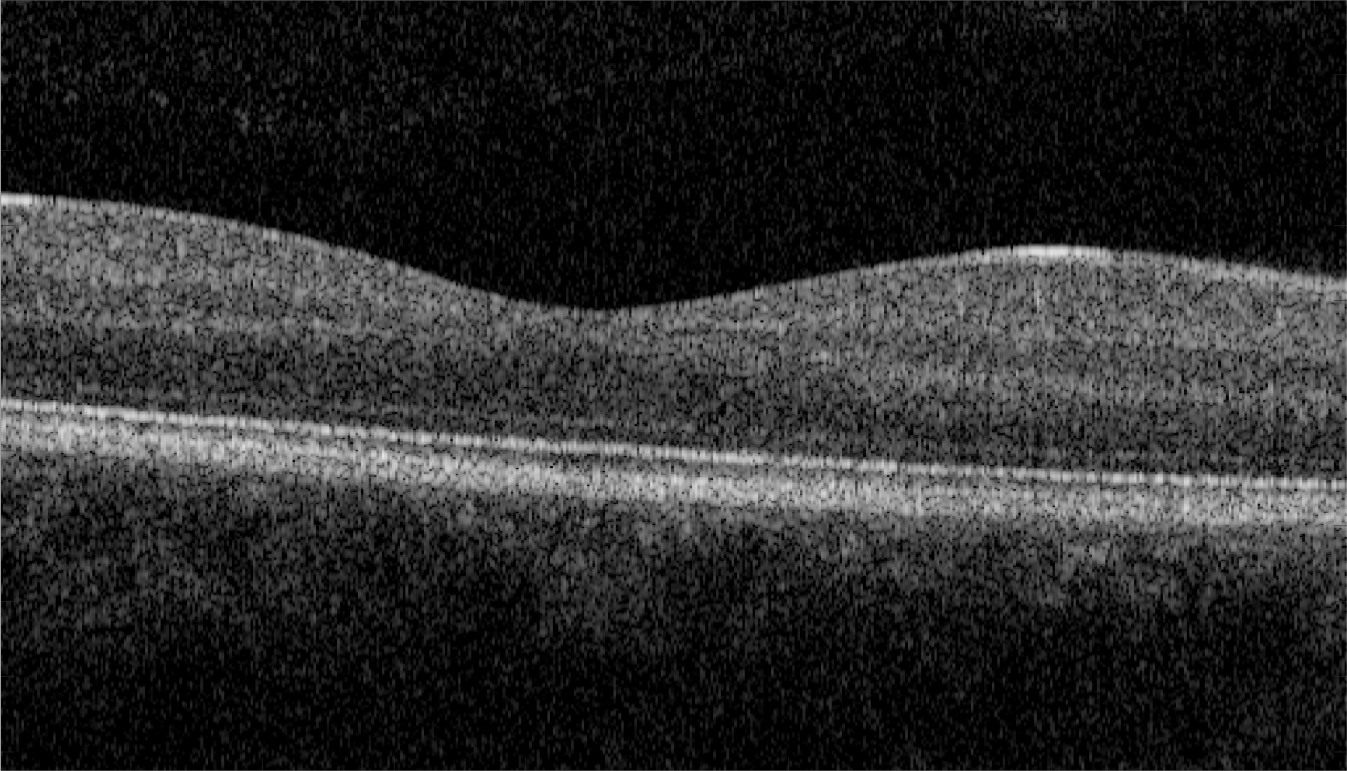
\includegraphics[width=0.7\linewidth]{img/chap3/Retina_Noisy_Bscan}
\caption[Imagen de la retina afectada por ruido de \textit{speckle}]{Imagen de la retina afectada por ruido de \textit{speckle}.}
\label{fig:Retina_Noisy_Bscan}
\end{figure}


%. El tamaño del \speckle en general puede contralarse a través de variaciones en la apertura numérica del sistema óptico, una apertura numérica menor produce patrones de \speckle relativamente grandes, mientras que una apertura numérica grande genera patrones más finos. 

La presencia de \speckle degradador reduce la calidad de las imágenes obtenidas por OCT, y en general, es deseable poder suprimir sus efectos, mientras se conserva la calidad de la imagen. El ruido causado por \speckle sobre una imagen se conoce como \emph{ruido multiplicativo}, y es un problema que se encuentra en múltiples técnicas de imagen coherente, por ejemplo, los radares de apertura sintética. A continuación, se relacionarán una técnica de filtrado proveniente de esta técnica de imagen, y que muestra un alto potencial para eliminar ruido en el caso de OCT.


\section{Del filtrado de \textit{speckle} en SAR a OCT}
\label{sec:from_SAR_to_OCT}

Los radares de apertura sintética (SAR) son una tecnología que ha visto un amplio desarrollo en los últimos años, gracias a las ventajas que posee para producir imágenes de terrenos de varios cientos de kilómetros. Los SAR han sido ampliamente utilizados para el estudio de procesos dinámicos en la superficie de la Tierra, ya que tiene la característica de proveer imágenes con alta resolución (en el orden de $1mm$) que son independientes de la luz solar, la presencia de nubes en la atmósfera e incluso de las condiciones climáticas \cite{Oliver2004,Moreira2013}. Las imágenes SAR son capturadas a través de la medición del eco que se produce en ondas electromagnéticas al ser retroreflejadas por la superficie del terreno analizado. En este caso, las ondas electromagnéticas tienen una longitud de onda que se encuentra del orden de las ondas de radio, con tamaños que abarcan unos cuantos milímetros, lo que permite observar estructuras tales como casas, carreteras, árboles entre otras. Su funcionamiento es análogo al de OCT, por lo tanto, las imágenes son altamente susceptibles al ruido de \textit{speckle} generado principalmente por centros dispersores para la escala de trabajo, siendo estos rocas, hidrantes o estructuras de tamaños similares \cite{Moreira2013}. 

El ruido producido por \speckle degrada altamente las imágenes reconstruidas mediante SAR, y por consiguiente, ha sido un área de gran interés para técnicas de filtrado que preserven estructuras finas mientras se elimina la mayor cantidad de ruido posible, conservando la fidelidad en la imagen filtrada \cite{Novak1990,Lopes2010}. En este sentido, algunas técnicas de filtrado de \speckle han surgido en el contexto de SAR y se han extendido a otras técnicas de imagen coherente, tales como ultrasonido, resonancia magnética y OCT. Sin embargo, pese al desarrollo de esta área, hay múltiples técnicas de filtrado que muestran un alto potencial para su implementación en otras técnicas de imagen coherente y aun están pendientes por explorar.

Inspirados por los resultados obtenidos por Lucas \etal \cite{Lucas2014} en la supresión de ruido por \speckle para los datos provenientes de la luna de Saturno Titan y capturados con la sonda Cassini-Huygens\footnote{Más información en \url{https://saturn.jpl.nasa.gov/mission/spacecraft/huygens-probe/}}, se decidió adaptar ese algoritmo de filtrado a OCT. Titan\footnote{Una imagen con la superficie de Titan filtrada puede encontrarse en \url{http://dralucas.geophysx.org/res.html}} es de alto interés científico por sus características hidrológicas, en donde destacan grandes lagos de metano, montañas de hielo y lluvias de metano en la superficie. Cabe resaltar que a la fecha, todavía se analiza la información enviada por la sonda, y que actualmente la NASA busca investigadores que trabajen con este tipo de datos para ayudar a develar la información hidrográfica que se encuentra en los datos adquiridos. Nuestro objetivo es adaptar el método de filtrado que emplean Lucas \etal para filtrar las imágenes provenientes del Cassini, para usarlo en el filtrado de datos adquiridos mediante OCT, y que de manera similar se encuentran altamente alterados por la presencia de ruido de \textit{speckle}, este algoritmo corresponde a una extensión del \textit{non-local means} (\textit{NL-Means}) mencionado anteriormente. Aunque al inicio de esta investigación, apareció la primera publicación en la cual se emplea \nlmeans en OCT por Yu \etal \cite{Yu2016}, nuestra motivación es poder extender esta técnica para emplear los datos tridimensionales que se adquieren con OCT, y con ello aprovechar mejor los datos disponibles al realizar el posprocesamiento.

%Inspirados por los resultados obtenidos por Lucas \etal \cite{Lucas2014} para la supresión de ruido por \speckle en datos provenientes de la sonda Cassini-Huygens\footnote{Una imagen de Titan filtrada puede encontrarse en \url{http://dralucas.geophysx.org/res.html}} en exploraciones topográficas de Titan, iniciadas en 2005, y cuyo objetivo es develar un mapa de esta luna de Saturno, se decidió emplear el algoritmo de filtrado empleado para las imágenes obtenidas de la sonda Cassini-Huygens. Cabe resaltar que a la fecha, todavía se analiza la información enviada por la sonda, y que actualmente la NASA busca investigadores que trabajen con este tipo de datos para ayudar a develar la información hidrográfica que se encuentra en lo datos enviados desde la sonda. Nuestro objeto es adaptar el método de filtrado que emplean Lucas \etal para filtrar las imágenes provenientes del Cassini, para ser empleado en el filtrado de datos provenientes de OCT, y que de manera similar se encuentran altamente alterados por la presencia de ruido de \speckle. Aunque al inicio de esta investigación, apareció la primera publicación en la cual se emplea \nlmeans para OCT, nuestra motivación es poder extender esta técnica de filtrado para el caso de datos en tres dimensiones, y poder de esta forma aprovechar mejor los datos disponibles en OCT.

\subsection{Principios del \textit{Non-Local Means}}

La técnica de filtrado espacial \nlmeans fue inicialmente propuesta por Baudes \etal \cite{Baudes2005} en el año 2005, \nlmeans aprovecha la redundancia existente en una imagen natural para realizar el filtrado de los datos, esto quiere decir que es posible encontrar una aproximación del ruido y sus características, así como una estimación de la imagen sin ruido empleando unicamente las propiedades intrínsecas de la imagen. En \nlmeans la redundancia de la imagen se aprovecha mediante la comparación de una pequeña zona con sus vecinos, en donde se espera que éstos sigan una forma y estructura definida, así que en lugar emplear unicamente píxeles, se utilizan pequeñas regiones de la imagen. En este contexto, si se tomaran pequeñas ventanas en la imagen, es posible encontrar múltiples zonas similares a lo largo de una región de búsqueda. La Fig.~\ref{fig:lennaPatches} muestra una imagen en donde las zonas indicadas como $\Delta_s$ claramente siguen una distribución espacial similar a las zonas indicadas como $\Delta_{t_1}$ y $\Delta_{t_2}$, con la diferencia de encontrarse a una distancia $\alpha_1$ y $\alpha_2$ de la zona central respectivamente. La región $\Delta_{t_3}$ a una distancia $\alpha_3$ por el contrario, no sigue la distribución de la imagen en $\Delta_s$, pero puede aportar con otro tipo de estadísticas tales como la varianza del ruido.% Empleando esta información y un criterio de similaridad, es posible encontrar la imagen real subyacente en los datos ruidosos.

Para encontrar la información no ruidosa $\nu_s$ en un punto $s$ de un espacio $\Omega$, tal que $s\in \Omega$ y $\Omega$ es del tamaño de la imagen, mediante una estimación $\hat{R}_s$ en base al conjunto de datos ruidosos $R_s$\footnote{Nótese que $\nu_s$ es el conjunto de datos libres de ruido, sin embargo, este conjunto no es posible de obtener, por lo que el filtrado realiza una estimación $\hat{R}_s$ que está directamente relacionada con $\nu_s$.}, \nlmeans emplea una vecindad $\Psi_s$ con $k$ miembros alrededor de un pixel central $s$, tal que una ventana $\Delta_{s}$ centrada en $s$ es comparada con una ventana $\Delta_t$ en todos los puntos $t\in k$ de la vecindad, como se ejemplifica en la Fig.~\ref{fig:patches}. Las ventanas $\Delta_s$ y $\Delta_t$ se denominan ventanas de similaridad, y corresponden a aquellas zonas comparadas, mientras que la vecindad $\Psi_s$ se le denomina ventana de búsqueda y determina la cantidad de vecinos que se compararán. Todas las posibles ventanas en los puntos $t$ se emplean para estimar el valor del pixel $\hat{R}_s$ de la imagen sin ruido. La comparación de un pixel central con sus vecinos, se regula a través de un criterio de \emph{similaridad}, que determina el grado de relación existente entre las zonas comparadas en la ventana de búsqueda.

\begin{figure}[!ht]
	\centering
	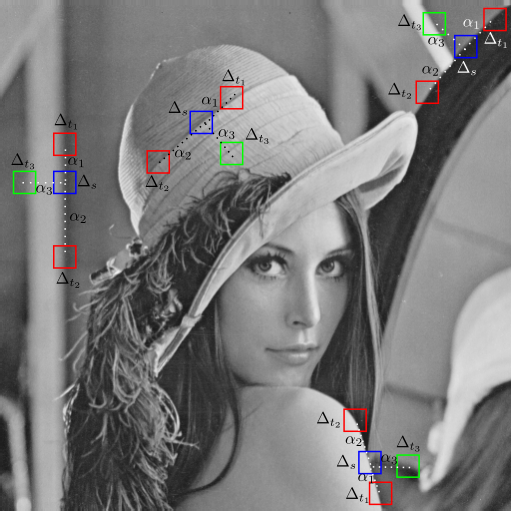
\includegraphics[width=0.5\linewidth]{img/chap3/lennaPatches}
	\caption[Comparación de ventanas en imagen natural.]{Comparación de ventanas en una imagen natural, las ventanas azules centradas siguen la misma distribución de aquellas regiones en rojo, por lo tanto, esta información permite realizar el filtrado de la imagen; este es el concepto en el cual se basa \textit{NL-Means}.}
	\label{fig:lennaPatches}
\end{figure}

\begin{figure}[!ht]
	\centering
	\includegraphics[width=0.5\linewidth]{img/chap3/patches}
	\caption[Dirección de escaneo de \textit{NL-Means}.]{Dirección de escaneo de \textit{NL-Means}, una ventana centradas en $s$ se evalúa con todos los vecinos centrados en $t$, y mediante un criterio de similaridad se realiza el filtrado de la imagen.}
	\label{fig:patches}
\end{figure}

En el contexto del estimador de pesos de máxima probabilidad (WMLE: \textit{weighted-maximum likelihood estimator}) \cite{Baudes2005}, el valor estimado del pixel sin ruido $\hat{R}_s$ se define a partir del conjunto de datos ruidosos $R_t$ como una suma promediada de pesos, esto es

\begin{equation}
\label{eq:R_WMLE}
\hat{R}_s = \frac{\sum_t w(s,t) R_t}{\sum_t w(s,t)},
\end{equation}

\noindent donde $w(s,t)$ corresponde al peso estimado para la ventana de similaridad $\Delta_s$ con respecto a la ventana $\Delta_t$ evaluada en todos los puntos $t\in k$. En la Eq.~\ref{eq:R_WMLE}, el numerador corresponde a la estimación de la similaridad entre las ventanas en la zona de búsqueda, mientras que el denominador es un factor de normalización para que la intensidad total de la imagen no se vea afectada por la suma de pesos. El problema de \nlmeans se encuentra justamente en la definición de los pesos $w(s,t)$, ya que son quienes definen el valor estimado de cada pixel de la imagen. En la propuesta inicial de \textit{NL-Means}, los pesos dependen de un criterio de similaridad entre las zonas a comparar $\Delta_s$ y $\Delta_t$, y se calcula mediante las intensidades en cada una de las regiones; mientras que a su vez dependerá de la distancia $\alpha_k$ que hay entre las zonas $\Delta_s$ y $\Delta_t$, por lo tanto regiones más cercanas tienen un mayor peso que aquellas zonas alejadas de la ventana central. En la Fig.~\ref{fig:lennaPatches} los pesos de las zonas $\Delta_{t_1}$ en general serán mayores que aquellos de las zonas $\Delta_{t_2}$ al encontrarse más cerca de $\Delta_s$, adicionalmente, $\Delta_{t_3}$ debe tener un peso cercano a cero, ya que no sigue la distribución de la imagen en la ventana de similaridad $\Delta_s$.  El hecho de que en este algoritmo, las comparaciones se realicen en una ventana de búsqueda es lo que le otorga la característica no local.

Los pesos $w(s,t)$ se definen \cite{Baudes2005} entonces como
\begin{equation}
\label{eq:nlmeans_normal_w}
w(s,t) = \exp\left(-\frac{1}{h} \sum_k \alpha_k \lvert R_{s,k}-R_{t,k} \rvert^2 \right),
\end{equation}

\noindent donde $\alpha_k$ define un kernel simétrico gaussiano centrado que regula los pesos de acuerdo a la distancia Euclideana que haya entre las zonas $\Delta_s$ y $\Delta_t$ e indica un disminución en la función con respecto a la distancia, $h$ determina el decaimiento de la función exponencial, actuando como un parámetro que regula el nivel de reducción al promediarse las ventanas $\Delta_s$ y $\Delta_t$. $R_{s,k}$ y $R_{s,t}$ son los $k$-ésimos vecinos miembros de las ventanas $\Delta_s$ y $\Delta_t$ respectivamente, éstos corresponden a las mediciones de intensidad experimental que se realizan. 

En general \nlmeans ha mostrado ser un algoritmo robusto para el filtrado de imágenes influenciadas por ruido blanco o ruido gaussiano, y es por ello que ha empleado y mejorado en diversas aplicaciones \cite{Mairal2009,Mahmoudi2005,Kervrann2007,Liu2008,Coupe2008}. Sin embargo, en el caso de ruido por \textit{speckle}, la implementación de \nlmeans no es directa, ya que el criterio de similaridad derivado por Baudes \etal \cite{Baudes2005} fue planteado para el caso de ruido blanco gaussiano. Una extensión de este algoritmo para el filtrado de imágenes provenientes de SAR fue propuesto por Deledalle \etal en 2009 \cite{Deledalle2009} y se conoce como \textit{probabilistic patch-based weights} (PPB), el cual es una extensión de \nlmeans adaptado para filtrar imágenes con ruido de \speckle provenientes de SAR, cuyas características generales difieren en gran medida del ruido blanco gaussiano, y adicionalmente requieren la consideración de diferentes propiedades asociadas con las causas del \textit{speckle}. 

%En el caso de \textit{speckle}, la función de densidad de probabilidad de que un pixel $s$ adquiera una amplitud determinada $A_s$ corresponde a una función del tipo Rayleigh (Sección~\ref{sec:principios_estadistica_speckle}), esta distribución se modifica cuando se promedian múltiples imágenes de una escena, este proceso corresponde al \multilooking, si se promedian $L$ imágenes, la función de densidad de probabilidad de Rayleigh se modifica a una conocida como distribución de Nakagami-Rayleigh, y sigue que

En el caso de \textit{speckle}, la función de densidad de probabilidad de que un pixel $s$ adquiera una amplitud determinada $A_s$ corresponde a una función del tipo Rayleigh (Sección~\ref{sec:principios_estadistica_speckle}). Uno de los procesos más comunes para la reducción de ruido por \textit{speckle}, consiste en el promediado incoherente de múltiples imágenes de la misma escena, esto es promediar varias imágenes de intensidad en un mismo punto, a este proceso se le denomina \textit{multilooking}. El promedio de $L$ imágenes modifica la función de densidad de probabilidad de adquirir una amplitud específica de una distribución de Rayleigh a una conocida como distribución de Nakagami o Nakagami-Rayleigh, que se describe como \cite{Deledalle2009}

%\cite{Coupe2009,Liu2010}
\begin{equation}
\label{eq:p_A_nakagami}
p_A(A) = \frac{2L^L}{\Gamma(L)R_s^L} A^{2L-1}_s \exp\left(-\frac{LA_s^2}{R_s}\right),
\end{equation}

\noindent donde $\Gamma()$ es la función gamma, $L$ se conoce como el número equivalente de vistas (ENL: \textit{equivalent number of looks}), $A_s$ es la amplitud en el campo imagen, y $R_s$ es la intensidad observada de la imagen $R_s = \lvert A_s \rvert^2$. Nótese que en el caso de $L=1$, la Eq.~\ref{eq:p_A_nakagami} es igual a la distribución de Rayleigh mencionada anteriormente, por lo tanto, la Eq.~\ref{eq:p_A_nakagami} es una generalización de la distribución de Rayleigh cuando se realiza \textit{multilooking}. En este contexto, la aproximación de la imagen libre de ruido se realiza también mediante un estimador de pesos de máxima probabilidad similar a la Eq.~\ref{eq:R_WMLE}, de la siguiente manera

\begin{equation}
\hat{R}(s) = \frac{\sum_t w(s,t) A^2(t)}{\sum_t w(s,t)}.
\end{equation}

Deledalle \etal \cite{Deledalle2009} describieron los pesos $w(s,t)$ a través de la combinación de un criterio de similaridad análogo al obtenido por Baudes \etal pero en el caso de ruido causado por \textit{speckle}, añadiendo también, una extensión iterativa al algoritmo. En ésta, se considera la probabilidad de que una zona filtrada $\hat{R}_{s,k}$ corresponda efectivamente a la imagen sin ruido al avanzar las iteraciones del algoritmo. Considerando la extensión del \nlmeans con PPB, y asumiendo que las imágenes se capturan unicamente una vez ($L=1$), los pesos en una iteración $i$ se definen como \cite{Deledalle2009}


\begin{equation}
\label{eq:nlmeans_w}
w(s,t) = \exp \left[-\sum_{k} \left( \frac{1}{h} \log \left(\frac{A_{s,k}}{A_{t,k}} + \frac{A_{t,k}}{A_{s,k}}\right) + \frac{1}{T} \frac{\big\lvert\hat{R}^{i-1}_{s,k} - \hat{R}^{i-1}_{t,k}\big\rvert^2}{\hat{R}^{i-1}_{s,k}\hat{R}^{i-1}_{t,k}} \right)\right].
\end{equation}

Los dos términos que aparecen en la sumatoria de la Eq.~\ref{eq:nlmeans_w} tienen el siguiente significado: $log\left(\frac{A_{s,k}}{A_{t,k}} + \frac{A_{t,k}}{A_{s,k}}\right)$ es el criterio de similaridad obtenido para el caso de ruido por \speckle análogo al mostrado en la Eq.~\ref{eq:nlmeans_normal_w} para el caso de ruido blanco gaussiano; el segundo término $\frac{\big\lvert\hat{R}^{i-1}_{s,k} - \hat{R}^{i-1}_{t,k}\big\rvert^2}{\hat{R}^{i-1}_{s,k}\hat{R}^{i-1}_{t,k}}$ expresa la probabilidad de que las dos zonas filtradas $\hat{R}^{i-1}_{s,k}$ y $\hat{R}^{i-1}_{t,k}$ efectivamente posean las características de la imagen sin ruido luego del filtrado en la iteración $i$, y contribuyen a partir de la segunda iteración para regular el grado de filtrado en las siguientes iteraciones del algoritmo. Estos dos términos se encuentra regidos por los parámetros $h$ y $T$: el parámetro $h$ cumple la función de regular la cantidad de filtrado sobre la imagen, mientras que el parámetro $T$ indica la fidelidad de datos entre iteraciones, esto es qué tan homogénea debe ser la imagen para considerarse como filtrada en la siguiente iteración. Una discusión extendida de los parámetros $h$ y $T$, y su importancia puede consultarse en \cite{Polzehl2006}. En una versión no iterativa del algoritmo, $T\rightarrow\infty$, y la Eq.~\ref{eq:nlmeans_w} corresponde a los pesos solamente dependientes del criterio de similaridad adaptados para el caso de ruido por \textit{speckle}. Finalmente, la Eq.~\ref{eq:nlmeans_w} se considera completamente \textit{no local} ya que no se penaliza de ninguna manera la distancia $\alpha_k$ entre las ventanas de similaridad.

\subsection{Implementación y resultados obtenidos con \textit{Non-Local Means} con PPB}
\label{sec:imple_result_nlmeansPPB}

El algoritmo de la implementación de \nlmeans con PPB se presenta en el Algoritmo~\ref{alg:nlmeansppb}, en donde a partir de la imagen ruidosa, el tamaño de la ventana de búsqueda y de similaridad, la cantidad de iteraciones y los parámetros $h$ y $T$ se calculan los pesos en cada pixel para obtener la imagen filtrada. Una particularidad que tiene \nlmeans se encuentra en la evaluación de los pesos en el pixel central $s=t$, en donde el criterio de similaridad tiende a producir \textit{sobrepeso} comparado con sus vecinos, esto se debe a que las zonas $\Delta_s$ y $\Delta_t$ son iguales cuando $t=s$, y como consecuencia de esto, el criterio de similaridad es máximo. Una opción para corregir este problema, consiste en omitir el pixel central y considerar el peso de éste como el máximo de la ventana de búsqueda, duplicando el mayor de los pesos encontrados, como lo sugiere \cite{Zhang2014}. La última consideración que debe tenerse en la implementación del algoritmo, es que los tamaños de las ventanas siempre deben ser impares para garantizar una región central donde se comparen de manera simétrica las ventanas de similaridad.


\begin{algorithm}
	\begin{tabularx}{0.8\textwidth}{l}
		
		%	\hline
		\textbf{Entrada:} datos ruidosos $R_s$, ventana de búsqueda $W$, ventana\\
		de similaridad $\Delta$, iteraciones $i$, parámetros $h$ y $T$.\\
		\hline
		\hspace*{0.6cm}\textbf{Inicio:} Calcular los pesos correspondientes de cada pixel $s$ en \\
		\hspace*{0.6cm}cada iteración $i$\\
		\hspace*{0.6cm}\textbf{Para} $n = 1 \hspace*{0.2cm} hasta \hspace*{0.2cm} i$\\
		\hspace*{0.9cm} \textbf{Para} $todo \hspace*{0.2cm} punto \hspace*{0.2cm} s$ \textbf{hacer}\\
		\hspace*{1.1cm} Tomar ventana de similaridad $\Delta_s$ de referencia en $s$ con $R_s$\\
		\hspace*{1.1cm} \textbf{luego} calcular vecinos $\Psi_s$ con $W$.\\
		\hspace*{1.1cm} \textbf{Fijar} $w_{max} =w_{tot} = 0$.\\
		\hspace*{1.1cm} \textbf{Para} $t\in \Psi_s$ \textbf{hacer}\\
		\hspace*{1.3cm} Tomar ventana de similaridad $\Delta_t$ \textbf{luego}\\
		\hspace*{1.3cm} calcular peso $w$, con la Eq. \ref{eq:nlmeans_w}.\\
		\hspace*{1.3cm} \textbf{Si} $t = s$\\
		\hspace*{1.5cm} \textbf{Continuar}\\
		\hspace*{1.3cm} \textbf{FinSi}\\
		\hspace*{1.3cm} \textbf{Si} $w > w_{max}$ \textbf{entonces}\\
		\hspace*{1.5cm} \textbf{Fijar} $w_{max} = w$\\
		\hspace*{1.3cm} \textbf{FinSi}\\
		\hspace*{1.3cm} $w_{tot} = w_{tot} + w$\\
		\hspace*{1.1cm} \textbf{FinPara}\\
		\hspace*{1.1cm} Calcular $\hat{R}_s$ con la Eq. \ref{eq:R_WMLE}, $w_{max}$ se duplica.\\
		\hspace*{0.9cm}\textbf{FinPara}\\
		\hspace*{0.9cm} $\hat{R}^{i-1}_s = \hat{R}_s$\\
		\hspace*{0.9cm} $n = n + 1$\\
		\hspace*{0.6cm}\textbf{FinPara}\\
		\hspace*{0.6cm}\textbf{Salida:} Retornar $\hat{R}_s$.\\
		%	\hline	
		
	\end{tabularx}
	\caption{Implementación del \nlmeans con PPB.}
	\label{alg:nlmeansppb}
\end{algorithm}


En la literatura \cite{Deledalle2009,Baudes2005} se recomiendan los siguientes parámetros para el filtrado: las ventanas de similaridad $\Delta_s$ y $\Delta_t$ deben tener un tamaño $\Delta = 7 \times 7$, la ventana de búsqueda $\Psi_s$ un tamaño $W = 21\times 21$, y cuatro iteraciones en el algoritmo $i = 4$. Adicionalmente, una ventaja que tiene la versión iterativa del \textit{NL-Means}, es que permite regular el filtrado de las estructuras finas en las imágenes variando el tamaño de la ventana de búsqueda en la primera iteración \cite{Deledalle2009}, de forma que ventanas más pequeñas tienden a preservar mejor estructuras finas, aunque filtran el ruido en un menor proporción; ventanas más grandes tienden a emborronar regiones de la imagen a cambio de reducir la varianza del ruido y homogeneizar estructuras. %Para los resultados, en la primer iteración, la ventana de búsqueda tuvo un tamaño $W^{(1)} = 7\times7$.
%En una versión no iterativa del algoritmo, $T\rightarrow\infty$ y la Eq.~\ref{eq:nlmeans_w} son los pesos obtenidos para el caso inicial del \textit{NLMeans}, pero adaptados para el caso de ruido de \speckle, adicionalmente, esta extensión se considera completamente no local, ya que no penaliza la distancia que haya entre las ventanas $\Delta_s$ y $\Delta_t$ evaluadas.

Las pruebas experimentales fueron realizadas con un volumen de $512\times512\times256$ [las dimensiones se consideran como $(Z,X,Y)$] con datos tomados en la retina de un paciente, adquiridos con un sistema de OCT comercial, el \textit{Spectralis} de la compañía \textit{Heidelberg Engineering}\footnote{Más información: \url{https://business-lounge.heidelbergengineering.com/int/products/spectralis/}}, los cuales fueron suministrados por el \textit{Wellman Center for Photomedicine}. Sin embargo, para estas pruebas se tomó una sección del volumen de $512\times512$ en $Y=128$ para realizar el filtrado. Es importante mencionar que en OCT la dirección del eje de escaneo rápido corresponde a $X$, mientras que el eje de escaneo lento es $Y$, y al mencionar imágenes se refieren a los datos del plano $ZX$, denominados anteriormente como escaneos tipo B. La imagen que representa los resultados, proviene de la sección transversal de la retina centrada en la fóvea, y muestra una imagen de las capas que la retina posee alrededor de la fóvea, tales como los fotoreceptores en la capa más brillante o los coroides en la capa inferior [Fig.~\ref{subfig:ima_nsy_nlmeansPPB}]. En la Fig.~\ref{fig:ima_filt_nlmeansPPB} se muestra el resultado obtenido para la imagen proveniente del sistema comercial de OCT. La Fig.~\ref{subfig:ima_nsy_nlmeansPPB} corresponde a la imagen ruidosa, la cual se ve fuertemente alterada por la presencia del ruido por \textit{speckle}, de hecho, algunas de las capas menos reflectivas que posee la retina no son diferenciables ya que el ruido degrada la calidad de la imagen, un ejemplo de esto es la región de los coroides, en donde es difícil diferenciar su estructura. La Fig.~\ref{subfig:ima_nsy_nlmeansPPB_multilook} es el promedio de cuatro imágenes con diferentes realizaciones de \speckle de la misma escena, en este caso se aprecia una mejora en la calidad de la imagen debido a que la presencia del ruido se reduce notoriamente, sin embargo, aun se alcanza a percibir ruido ya que este proceso no elimina completamente el \textit{speckle}. La desventaja fundamental de realizar \multilooking es que se debe extender el tiempo de captura de datos en el paciente, lo que deriva en posibles movimiento entre escaneos B, o en algunas aplicaciones de OCT, riesgos para la salud del paciente. La Fig.~\ref{subfig:ima_filt_nlmeansPPB_gaussian} es un filtrado gaussiano de la imagen ruidosa [Fig.~\ref{subfig:ima_nsy_nlmeansPPB}], como en este caso se tiene ruido por \speckle es necesario convertir primero la imagen a escala logarítmica, en donde el ruido por \speckle es aditivo y luego realizar el filtrado, aun así, no hay una mejora sustancial en la calidad de la imagen. Por último, la Fig.~\ref{subfig:ima_filt_nlmeansPPB} es el resultado del proceso de filtrado con los parámetros recomendados por la literatura, y tomando $h = 16$ y $T = 19$, esta imagen presenta alta atenuación del ruido, y permite diferenciar fácilmente las diferentes capas de la retina. No obstante, una inspección detenida de la imagen muestra también algunos problemas respecto al filtrado, por ejemplo el efecto \textit{acuarela} que se percibe, y la presencia de estructuras periódicas finas que aparecen como artefactos.

\begin{figure}[ht!]
	\centering
	\subfigure[Imagen ruidosa.]{\label{subfig:ima_nsy_nlmeansPPB}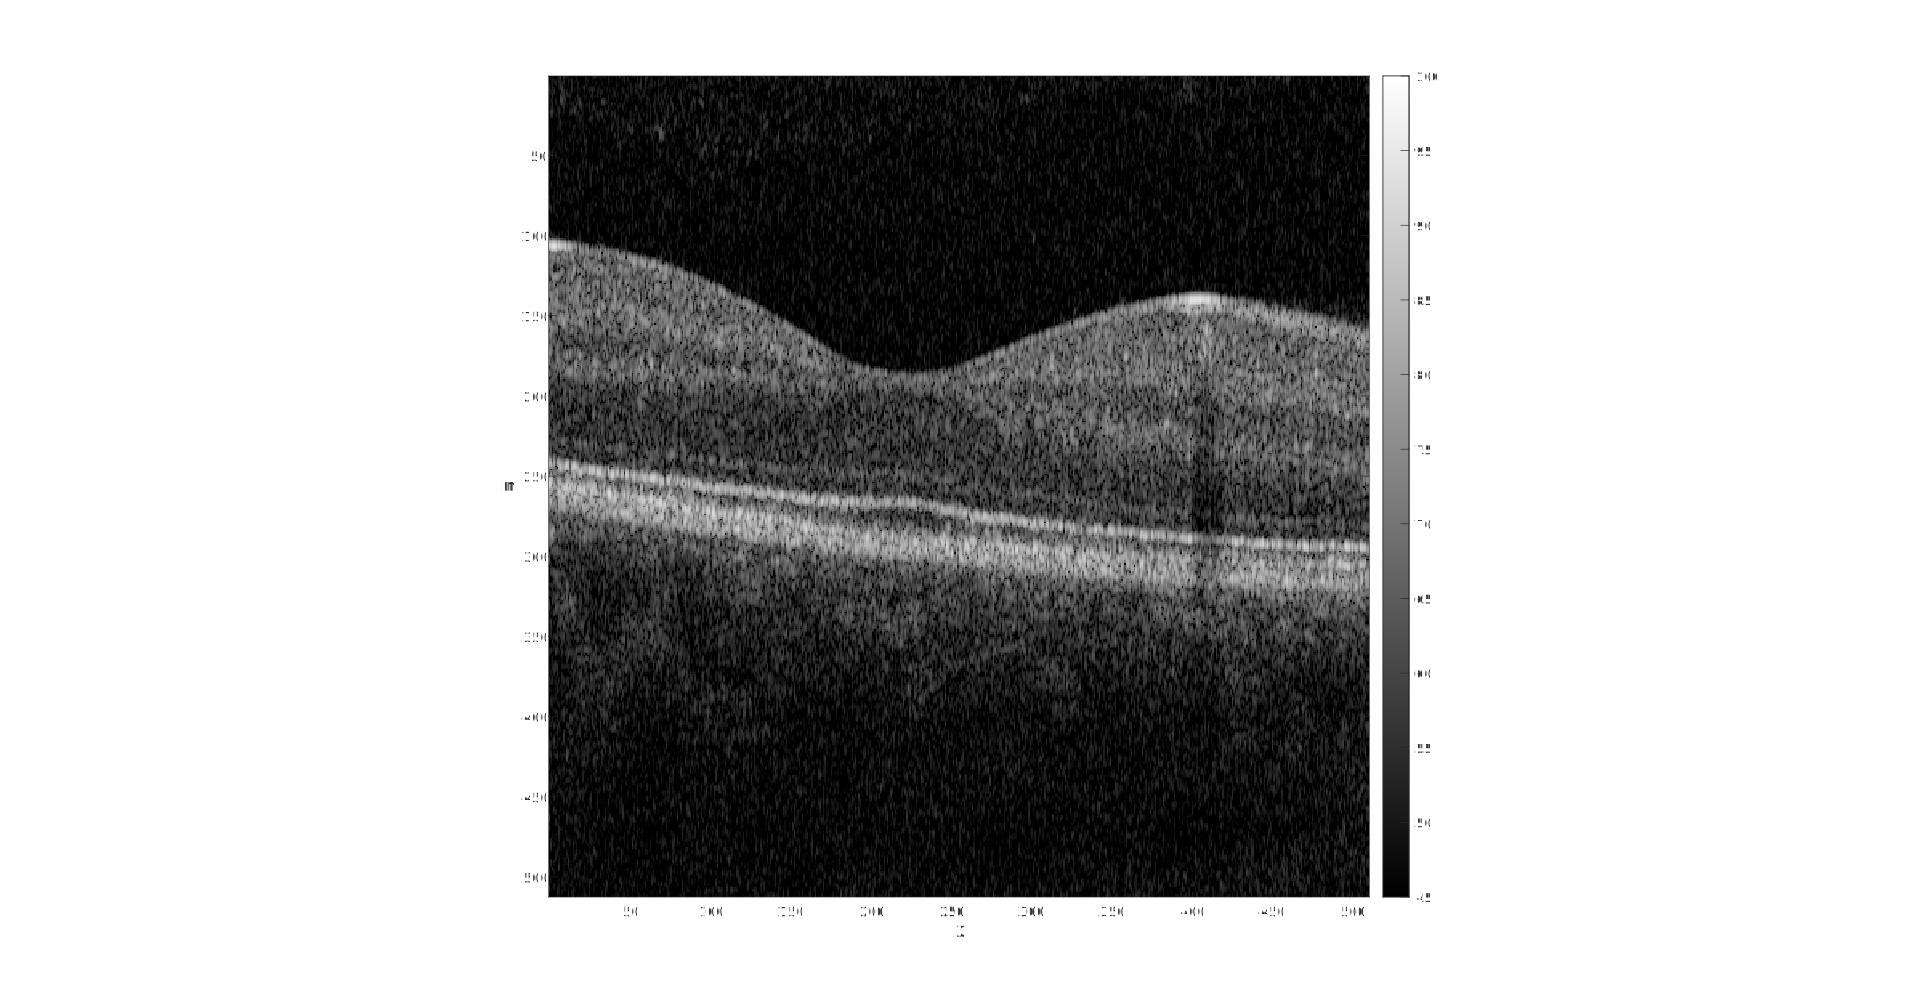
\includegraphics[width=0.4\linewidth]{img/chap3/Retinal_NoisyImage_Bscan128}}
	\subfigure[Imagen resultante del promedio de cuatro imágenes de la misma escena.]{\label{subfig:ima_nsy_nlmeansPPB_multilook}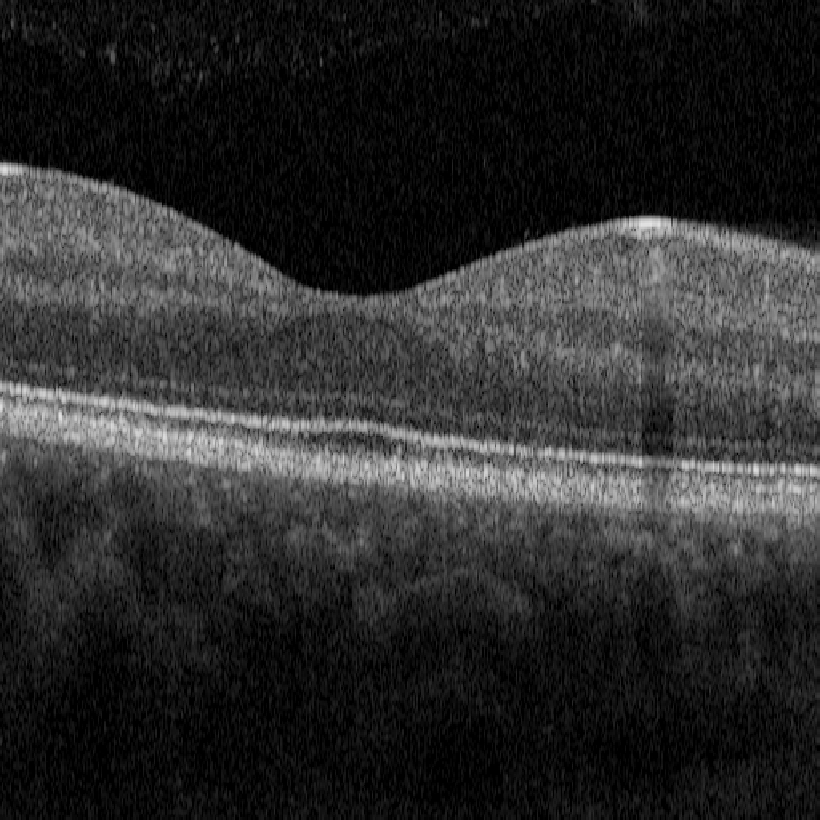
\includegraphics[width=0.4\linewidth]{img/chap3/Retinal_NoisyImage4Mlooks_Bscan128}}
	\subfigure[Imagen filtrada con un filtro gaussiano de tamaño $(7x7)$.]{\label{subfig:ima_filt_nlmeansPPB_gaussian}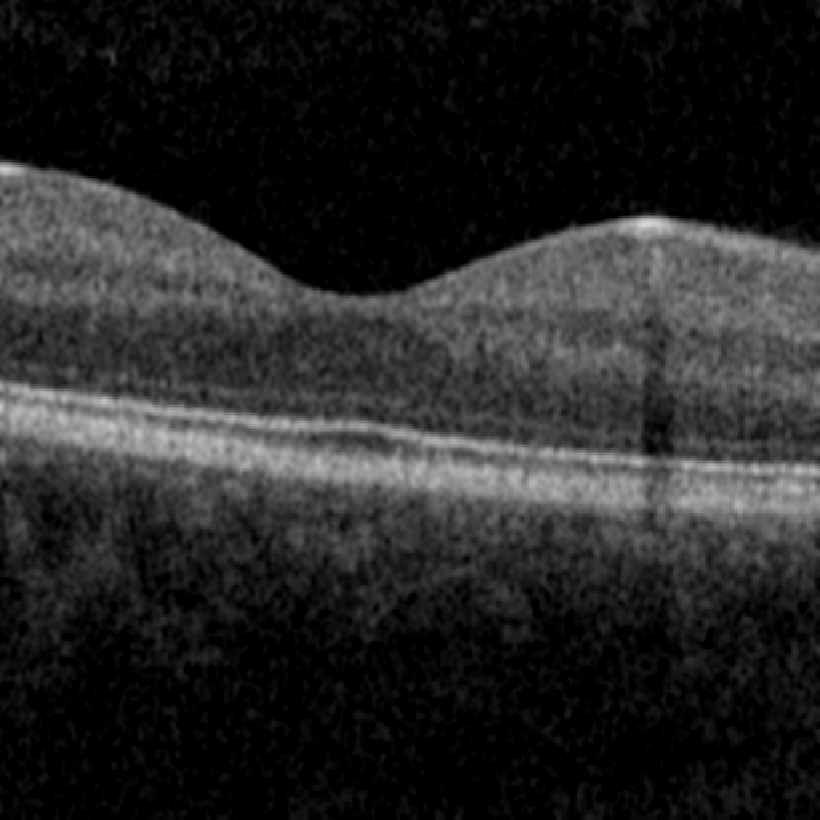
\includegraphics[width=0.4\linewidth]{img/chap3/Retinal_GaussFilter_sigma1d5_Image_Bscan128}}	
	\subfigure[Imagen filtrada mediante \nlmeans con PPB.]{\label{subfig:ima_filt_nlmeansPPB}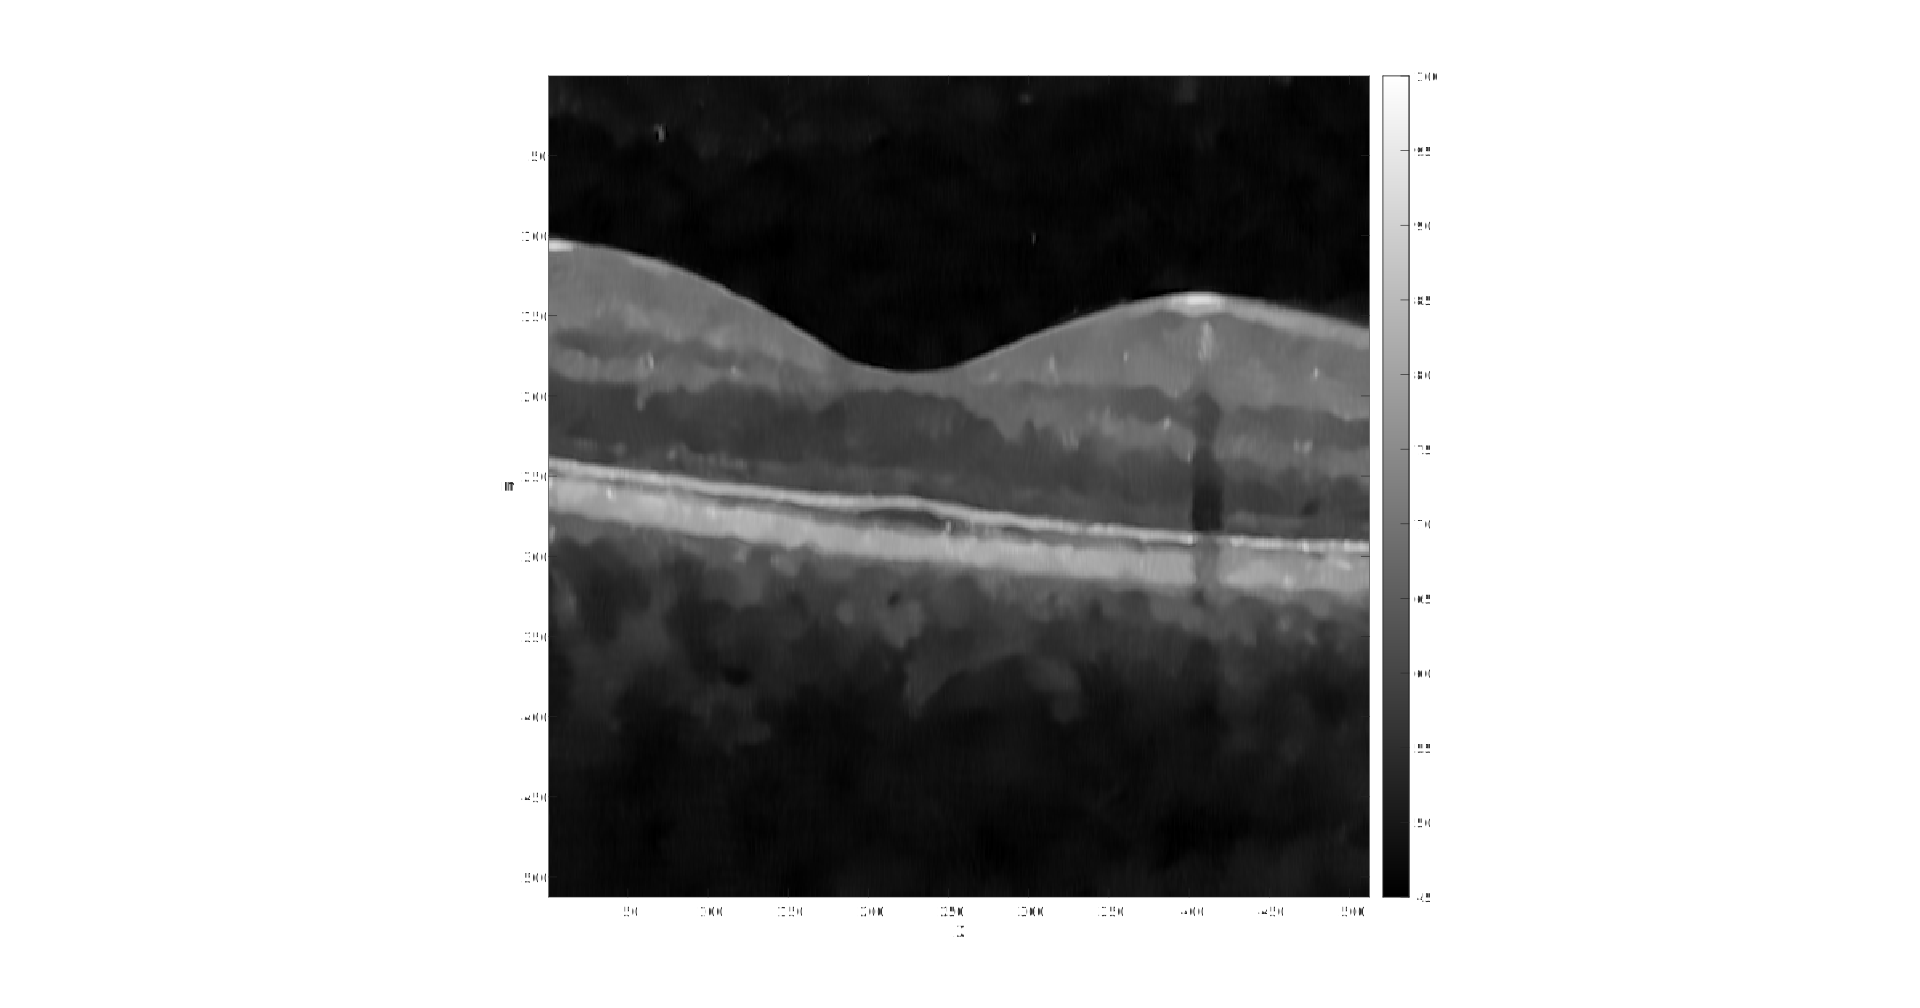
\includegraphics[width=0.4\linewidth]{img/chap3/Retinal_NLMeansIterativo_Bscan128}}
	\caption[Resultado del filtrado de una imagen proveniente de un sistema comercial de OCT para la retina]{Resultado del filtrado de una imagen proveniente de un sistema comercial de OCT para la retina. (a) es la imagen ruidosa capturada donde la presencia del \speckle degrada fuertemente la calidad de la imagen, (b) es el promedio incoherente de cuatro imágenes de la misma región, aunque en este caso hay una mejora en la calidad de la imagen, el ruido por \speckle sigue siendo notorio, (c) resultado del filtro gaussiano de la imagen (a) aunque hay una mejora, la imagen sigue teniendo una alta presencia de ruido, y (d) resultado obtenido con el filtrado mediante \nlmeans con PPB, el ruido por \speckle es altamente atenuado.}
	\label{fig:ima_filt_nlmeansPPB}
\end{figure}

Aunque los resultados de la Fig.~\ref{subfig:ima_filt_nlmeansPPB} muestran que hay una mejora en la calidad de la imagen y que \nlmeans con PPB elimina el ruido indeseado, no es una imagen óptima para ser presentada ante un especialista, quien es el usuario final de los datos luego del filtrado, esto debido a que la imagen pareciera ser sintética y no proveniente de un paciente. Nuestro siguiente objetivo fue mejorar el resultado obtenido con la implementación del \nlmeans con PPB a través de añadir pasos adicionales antes del filtrado. En ese orden de ideas, la primera propuesta que se hizo para mejorar el desempeño del algoritmo, fue la transformación de la imagen proveniente de OCT a una representación diferente, que se conoce como la \textit{representación en coeficiente de atenuación}. La segunda propuesta consistió en obtener y promediar dos imágenes a partir del conjunto de datos, esto es posible a través de la división del espectro medido en dos, y luego tomar sus respectivas transformadas de Fourier. Sin embargo, estas propuestas no mostraron una mejora en el desempeño del filtrado, por lo que se decidió modificar el funcionamiento de las ventanas de similaridad y búsqueda, haciendo uso de la información volumétrica disponible en OCT. En base a esto, se obtuvo que una modificación sobre las ventanas de similaridad y de búsqueda extendidas al caso tridimensional producen un mejor resultado del algoritmo. A continuación se profundizará en las pruebas realizadas y en la propuesta final.

\subsubsection{Representación de imágenes de OCT como coeficientes de atenuación}

La representación en coeficiente de atenuación es una manera alternativa de describir los datos proveniente de un sistema de OCT. El coeficiente de atenuación se puede entender como la reducción de la potencia en un haz que se propaga por un medio turbio, debido al esparcimiento y la absorción que éste experimenta \cite{Vermeer2013}. El coeficiente de atenuación depende de las características del medio, aportando información sobre su composición, es decir, un medio cuyo coeficiente de atenuación sea $5mm^{-1}$ produce un rápido decaimiento de la señal con respecto a la profundidad. La perdida de intensidad de la señal $I(z)$ detectada por el sistema de OCT en función de la profundidad $z$, puede describirse como

%Un medio cuyo coeficiente de atenuación sea grande, produce un rápido decaimiento de la señal con respecto a la profundidad. Como el coeficiente de atenuación depende de las características del medio, aporta información de su composición. 

\begin{equation}
 I(z) \propto e^{-2\mu z},
\end{equation}

\noindent donde $\mu$ es el coeficiente de atenuación y el factor $2$ surge por el viaje de ida y regreso del haz. Siguiendo el tratamiento de Vermeer \etal \cite{Vermeer2013}, una forma alterna de describir la imagen de intensidad de OCT, es a través de la imagen en coeficiente de atenuación, relacionadas de la siguiente manera

\begin{equation}
\label{eq:mu}
\mu (z) = \frac{I(z)}{2\int_{z}^{\infty} I(u)du},
\end{equation}

\noindent es decir, que el coeficiente de atenuación es proporcional a la intensidad registrada en una profundidad con respecto a la intensidad restante en toda la profundidad. Mediante una linearización de primer orden de la función $\log(1+x)$ y considerando la discretización de la imagen de OCT \cite{Vermeer2013}, la Eq.~\ref{eq:mu} puede reescribirse como 

\begin{equation}
\label{eq:mu_i}
\mu [i] \approx \frac{I[i]}{2\Xi \sum_{i+1}^{\infty}I[i]},
\end{equation}

\noindent donde $\Xi$ es el tamaño del pixel e $[i]$ representa los puntos discretos de la imagen. 

La representación en coeficiente de atenuación de la imagen ruidosa en la Fig.~\ref{subfig:ima_nsy_nlmeansPPB} se muestra en la Fig.~\ref{subfig:att_coef_nsy}. Las pruebas realizadas mediante la combinación de filtrado en la representación de coeficiente de atenuación, no mostraron una mejora en el resultado obtenido por medio de \nlmeans con PPB, de hecho, se observó que filtrar la imagen ruidosa en intensidad y luego convertirla a coeficiente de atenuación produce resultados muy similares a filtrar la imagen en términos del coeficiente de atenuación. La explicación de esto se encuentra sustentada en que la transformación integral que se realiza en la Eq.~\ref{eq:mu_i} no modifica la composición del ruido. El resultado del filtrado y posterior conversión a coeficiente de atenuación se presenta en la Fig.~\ref{subfig:att_coef_filt}. Como conclusión, la representación en coeficiente de atenuación no aportó modificaciones relevantes sobre el filtrado del ruido en la imagen, pero permitió ver como el filtrado es invariante ante en la conversión coeficiente de atenuación contra intensidad.

\begin{figure}[ht!]
	\centering
	\subfigure[Imagen ruidosa representada en coeficiente de atenuación.]{\label{subfig:att_coef_nsy}\includegraphics[width=0.4\linewidth]{img/chap3/CoeficientesAtenuacionCorregidos/singlelookAttCoeffNsy}}
	\subfigure[Imagen filtrada representada en coeficiente de atenuación.]{\label{subfig:att_coef_filt}\includegraphics[width=0.4\linewidth]{img/chap3/CoeficientesAtenuacionCorregidos/singlelookAttCoeffFilt}}
	\caption[Representación de imágenes en coeficientes de atenuación]{Representación de las imágenes ruidosa y filtrada en coeficiente de atenuación. (a) imagen ruidosa y (b) imagen filtrada.}
	\label{fig:att_coeff}
\end{figure}

\subsubsection{Obtención de dos imágenes a partir de un solo espectro}

La captura de los datos en sistemas de OCT en el dominio de Fourier como se mencionó en la Sección \ref{sec:int_baja_coh_fourier} se realiza a través del registro del patrón de interferencia en el dominio de las frecuencias, en este sentido, los datos capturados se convierten en imágenes mediante una transformada de Fourier. Debido a que el espectro de la señal contiene la información proveniente de todas las contribuciones, es posible dividir el espectro para obtener múltiples imágenes que contengan una cantidad reducida de información de la escena. Esto quiere decir, que desde un solo espectro pueden derivarse múltiples imágenes cuyas realizaciones de \speckle difieran, a través de la asignación de un ancho de banda diferente para cada una de las nuevas imágenes, sin embargo, este procedimiento tiene la desventaja de producir una pérdida de resolución asociada con la limitación del espectro para cada una de las imágenes. 

Como se muestra en la Fig.~\ref{subfig:dos_espectros_de_uno} a partir del espectro azul, dos nuevos espectros pueden ser derivados (rojo y amarillo), éstos comparten la información del espectro inicial en un ancho de banda diferente, por lo tanto, se tendrán diferentes características en la composición del \speckle de las imágenes derivadas al realizar las transformaciones. Si se toma un promedio de las imágenes derivadas del espectro inicial se reduce la presencia de ruido de \speckle de manera similar al promedio de múltiples imágenes de la misma escena. Este procedimiento puede ser útil, ya que como se mostró anteriormente, realizar un promediado incoherente de la misma imagen reduce significativamente el contraste del \speckle y facilita el filtrado de los datos. 

La Fig.~\ref{subfig:2spectra_mean_image} presenta el promedio de las dos imágenes obtenidas a partir de los espectros rojo y amarillo [Fig.~\ref{subfig:dos_espectros_de_uno}], la línea horizontal que aparece se debe a la presencia de artefactos causados por la pérdida de información en los espectros derivados, asimismo, se aprecia una perdida de los detalles tales como los bordes de la imagen. En la Fig.~\ref{subfig:2spectra_mean_image_filt} se encuentra el resultado de filtrar los nuevos datos, esta imagen no muestra una diferencia significativa con respecto a los filtrados realizados anteriormente, además tiene la desventaja de poseer una menor resolución. Esto permite concluir que intentar generar dos imágenes desde un espectro mediante un intercambio entre resolución y nivel de ruido no es una buena alternativa, ya que no se mejora el desempeño del filtrado y se tiene una reducción en la resolución de la imagen final.


\begin{figure}[h!]
	\centering
	\subfigure[Espectro medido para una línea A.]{\label{subfig:dos_espectros_de_uno}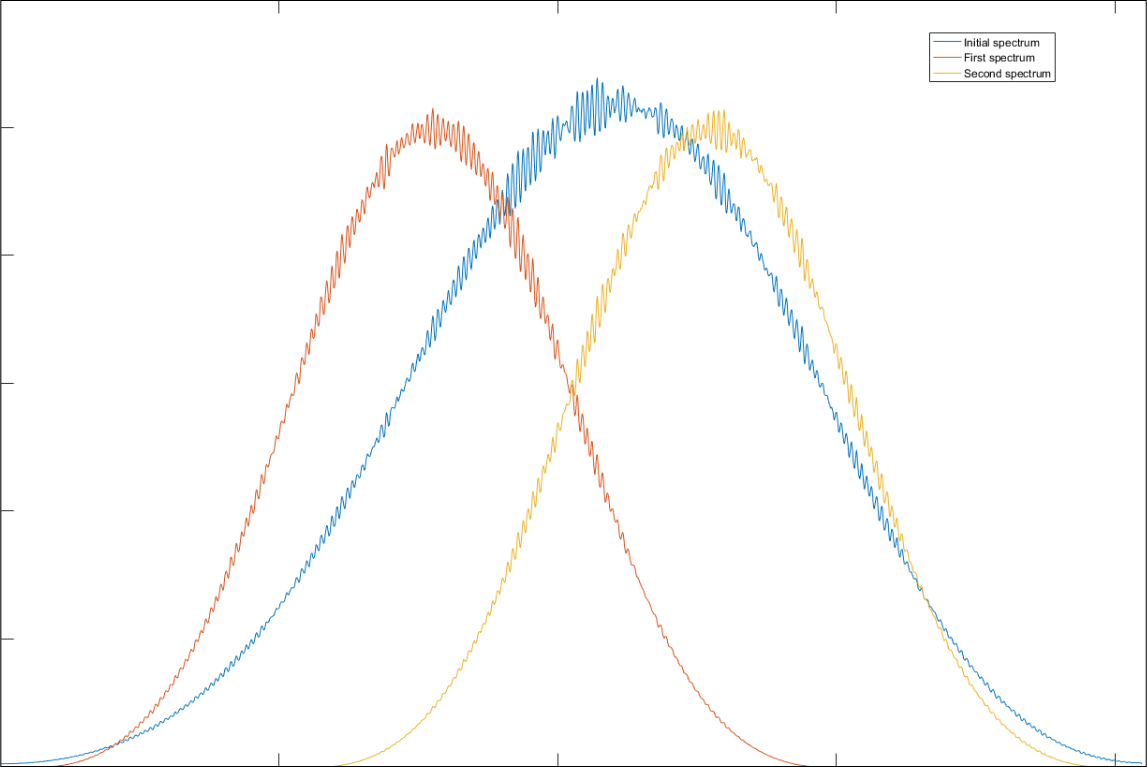
\includegraphics[width=0.4\linewidth]{img/chap3/espectros/EspectrosParticion}}\\
	\subfigure[Imagen obtenida del promedio de las dos subimágenes.]{\label{subfig:2spectra_mean_image}\includegraphics[width=0.4\linewidth]{img/chap3/espectros/imgFrom2SpectraNsy}}
	\subfigure[Imagen proveniente de los dos espectros filtrada.]{\label{subfig:2spectra_mean_image_filt}\includegraphics[width=0.4\linewidth]{img/chap3/espectros/imgFrom2SpectraFilt}}
	\caption[Generación de dos imágenes a partir de un espectro]{Obtención de dos imágenes a partir de un único espectro. (a) Los espectros rojo y amarillo se obtiene a partir de espectro azul, en ese caso, se producen dos imágenes con diferentes realizaciones de \textit{speckle} a cambio de una perdida en la resolución axial. (b) imagen ruidosa obtenida del promedio de los espectros amarillo y rojo. (c) imagen filtrada a partir del promedio de dos espectros partiendo de uno.}
	\label{fig:2images_from_one_spectra}
\end{figure}



\subsection{Modificación sobre \nlmeans propuesta (\textit{NL-Means-OCT})}

Las pruebas realizadas añadiendo transformaciones y pasos adicionales al \nlmeans con PPB no mostraron una mejora significativa en los resultados, por lo que luego de realizar múltiples pruebas con variaciones y distintas formas de filtrar, se llegó hasta un resultado que aprovecha y requiere la información volumétrica disponible en OCT. La modificación que se plantea consiste entonces en variar la forma en la que \nlmeans con PPB realiza el cálculo de los pesos entre las ventanas de similaridad al interior de la ventana de búsqueda. Para tal fin, se propone emplear una modificación del \nlmeans en tres dimensiones planteado por Lu \etal \cite{Lu2011} en donde la ventana de búsqueda es cúbica al igual que las ventanas de similaridad, en conjunto con la implementación bidimensional del \textit{NL-Means} con PPB presentada por Deledalle \etal \cite{Deledalle2009}, de la siguiente manera. Partiendo del escaneo propuesto en la Fig.~\ref{fig:patches}, en la cual las ventanas de similaridad $\Delta_s$ y $\Delta_t$, y la ventana de búsqueda $\Psi_s$ son cuadradas, se sugiere modificar las ventanas de similaridad para ser cúbicas, por lo tanto las zonas $\Delta_s$ y $\Delta_t$ adquirirán información sobre los vecinos en las tres dimensiones $(Z,X,Y)$, pero conservando la ventana de búsqueda bidimensional, esto permite filtrar los datos a lo largo de tres posibles planos $ZX$, $ZY$ y $XY$. Los cubos de similaridad $\Delta_s$ y $\Delta_t$ propuestos, así como la ventana de búsqueda $\Psi_s$ se ejemplifican en la Fig.~\ref{fig:Patches_propuesta}.

\begin{figure}
	\centering
	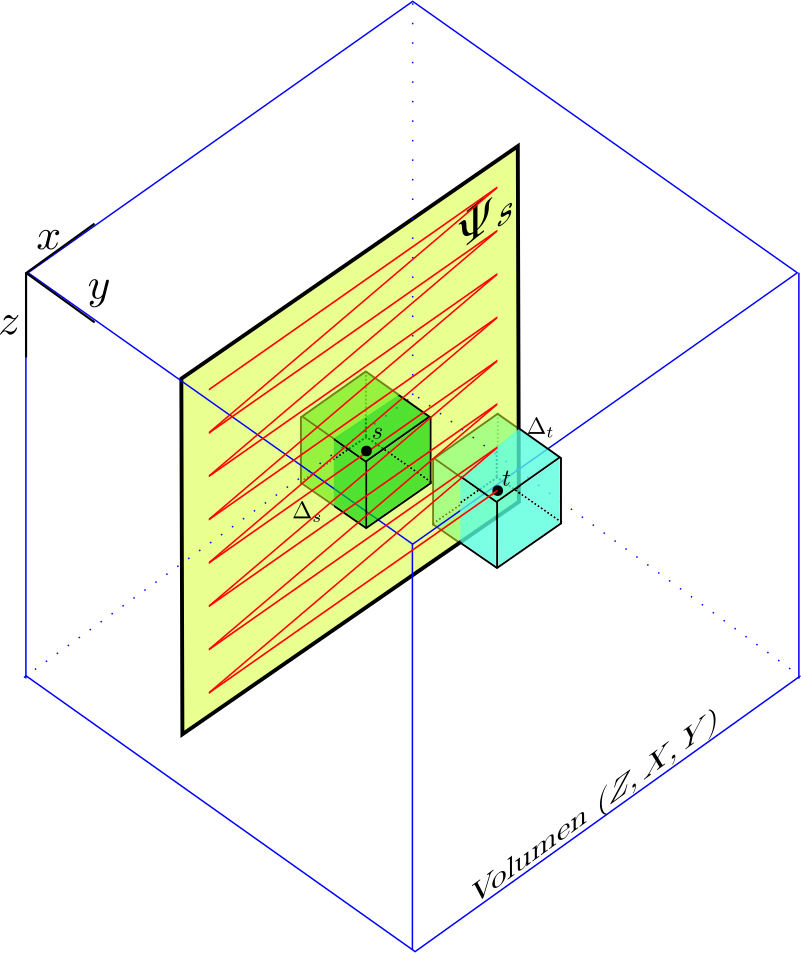
\includegraphics[width=0.4\linewidth]{img/chap3/Patches_propuesta}
	\caption[Modificación de las ventanas de similaridad y búsqueda propuesta.]{Modificación de las ventanas de similaridad y búsqueda propuesta. Las ventanas de similaridad son cubos que toman en cuenta información de sus vecinos, mientras se mantiene la ventana de búsqueda en el plano del eje rápido de escaneo $ZX$.}
	\label{fig:Patches_propuesta}
\end{figure}

%La idea es incrementar la cantidad de datos presente en las ventanas de similaridad, por lo que una mayor cantidad de información se emplea para comparar y por tanto, debe haber una mejora cuando se realiza el filtrado porque se emplean los patrones de \speckle como patrones volumétricos. 

La idea es incrementar la cantidad de datos presente en las ventanas de similaridad ya que son ellas quienes determinan los pesos para el filtro, así se espera una mejora cuando se realiza el filtrado porque se emplean las regiones de la imagen y los patrones de \speckle como volúmenes. La ventana de búsqueda se mantiene bidimensional, ya que si esta tuviese tres dimensiones el tiempo de computo para el algoritmo se vería incrementado en un factor de $\approx 5\times$, además se espera que en esta ventana se encuentre una cantidad suficiente de vecinos para realizar adecuadamente el filtrado, como lo hace \nlmeans con PPB. 

Las posibilidades del plano de orientación de la ventana de búsqueda también tienen una implicación sobre el filtrado, particularmente en el caso de OCT, en donde al tomar los datos experimentales por lo general hay movimientos indeseados que se dan por fuentes externas y producen desplazamientos entre las diferentes imágenes que conforman el volumen; cabe resaltar que éstos desplazamientos se aplican para una imagen entera. En ese orden de ideas, escoger como plano de filtrado aquel correspondiente al eje de escaneo rápido del sistema de OCT ($ZX$), reduce los problemas asociados con movimientos aleatorios causados por el paciente.

En cuanto al cálculo de los pesos también se propone una modificación a la Eq.~\ref{eq:nlmeans_w} utilizada en el \nlmeans con PPB, en este caso, se sugiere emplear una versión no iterativa del algoritmo, es decir, hacer que $T \rightarrow \infty$, y por tanto calcular los pesos $w(s,t)$ de la siguiente manera

\begin{equation}
\label{eq:w_propuesta}
w(s,t) = \exp \left[-\sum_{k} \frac{1}{h} \log \left(\frac{A_{s,k}}{A_{t,k}} + \frac{A_{t,k}}{A_{s,k}}\right) \right].
\end{equation}

\noindent La Eq.~\ref{eq:w_propuesta} es unicamente la adaptación de los pesos para el caso del ruido por \textit{speckle} aplicado a una ventana tridimensional. A esta propuesta se le denominará \textit{NL-Means-OCT}.

\section{Resultados obtenidos y aplicaciones}
\label{sec:resultado_filtrado}

% Con el algoritmo propuesto se realizó nuevamente el filtrado de los datos provenientes del sistema comercial de OCT para la retina, sin embargo, los resultados obtenidos muestran la ventaja del 

\subsection{OCT en la retina}
\label{subsec:oct_retinal}

En el caso de los datos obtenidos para la retina, se empleó el mismo conjunto de datos y un procedimiento similar al planteado en la Sección~\ref{sec:imple_result_nlmeansPPB}, pero tomando en cuenta los cambios propuestos sobre el algoritmo de filtrado, con los siguientes parámetros: tamaño de las ventanas (cubos) de similaridad $\Delta = 7\times7\times7$, tamaño de la ventana de búsqueda $W = 21\times21$ y parámetro de filtrado $h = 18$. A partir de estos criterios se filtró el volumen de $512\times512\times216$ con datos de la retina del paciente, en un computador Intel Core i-7 de $2.93GHz$ (4CPUs) y $6GB$ de memoria, el tiempo de procesamiento total de $69.3$ horas. El resultado obtenido con \nlmeansOCT comparado contra \nlmeans con PPB se presenta en la Fig.~\ref{fig:retinal_ima_nlemans_OCT}. La Fig.~\ref{subfig:retinal_ima_nsy} es igual a la presentada en la Fig.~\ref{subfig:ima_nsy_nlmeansPPB} y corresponde a la imagen afectada por ruido de \textit{speckle}, la Fig.~\ref{subfig:retinal_filtrado_nlmeansPPB} es el resultado obtenido empleando \nlmeans con PPB, la Fig.~\ref{subfig:retinal_filtrado_nlmeansOCT_ZX} representa el resultado obtenido usando \nlmeansOCT con la ventana de búsqueda orientada sobre el plano $ZX$, por último, la Fig.~\ref{subfig:retinal_filtrado_nlmeansOCT_ZY} es la imagen recuperada con \nlmeansOCT ubicando la ventana de búsqueda en el plano $ZY$. 

\begin{figure}[ht!]
	\centering
	\subfigure[Imagen ruidosa.]{\label{subfig:retinal_ima_nsy}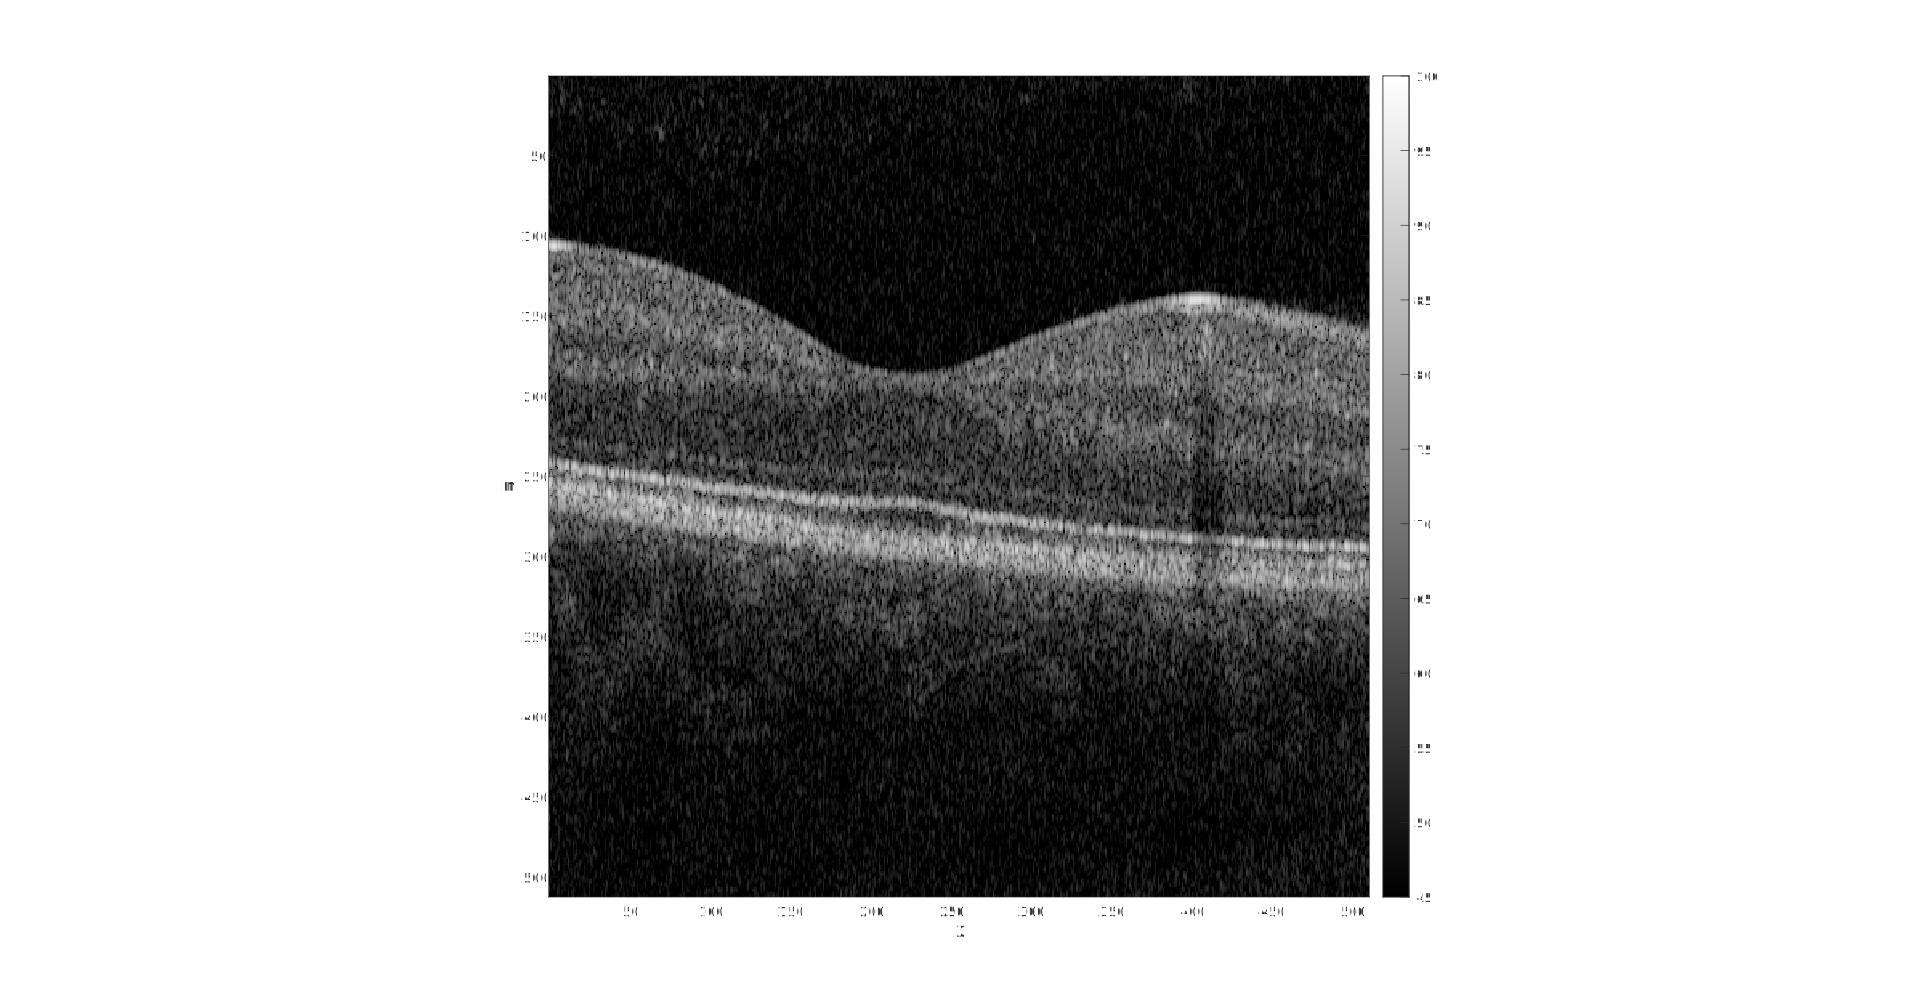
\includegraphics[width=0.49\linewidth]{img/chap3/Retinal_NoisyImage_Bscan128}}
	\subfigure[Filtrado con \nlmeans con PPB.]{\label{subfig:retinal_filtrado_nlmeansPPB}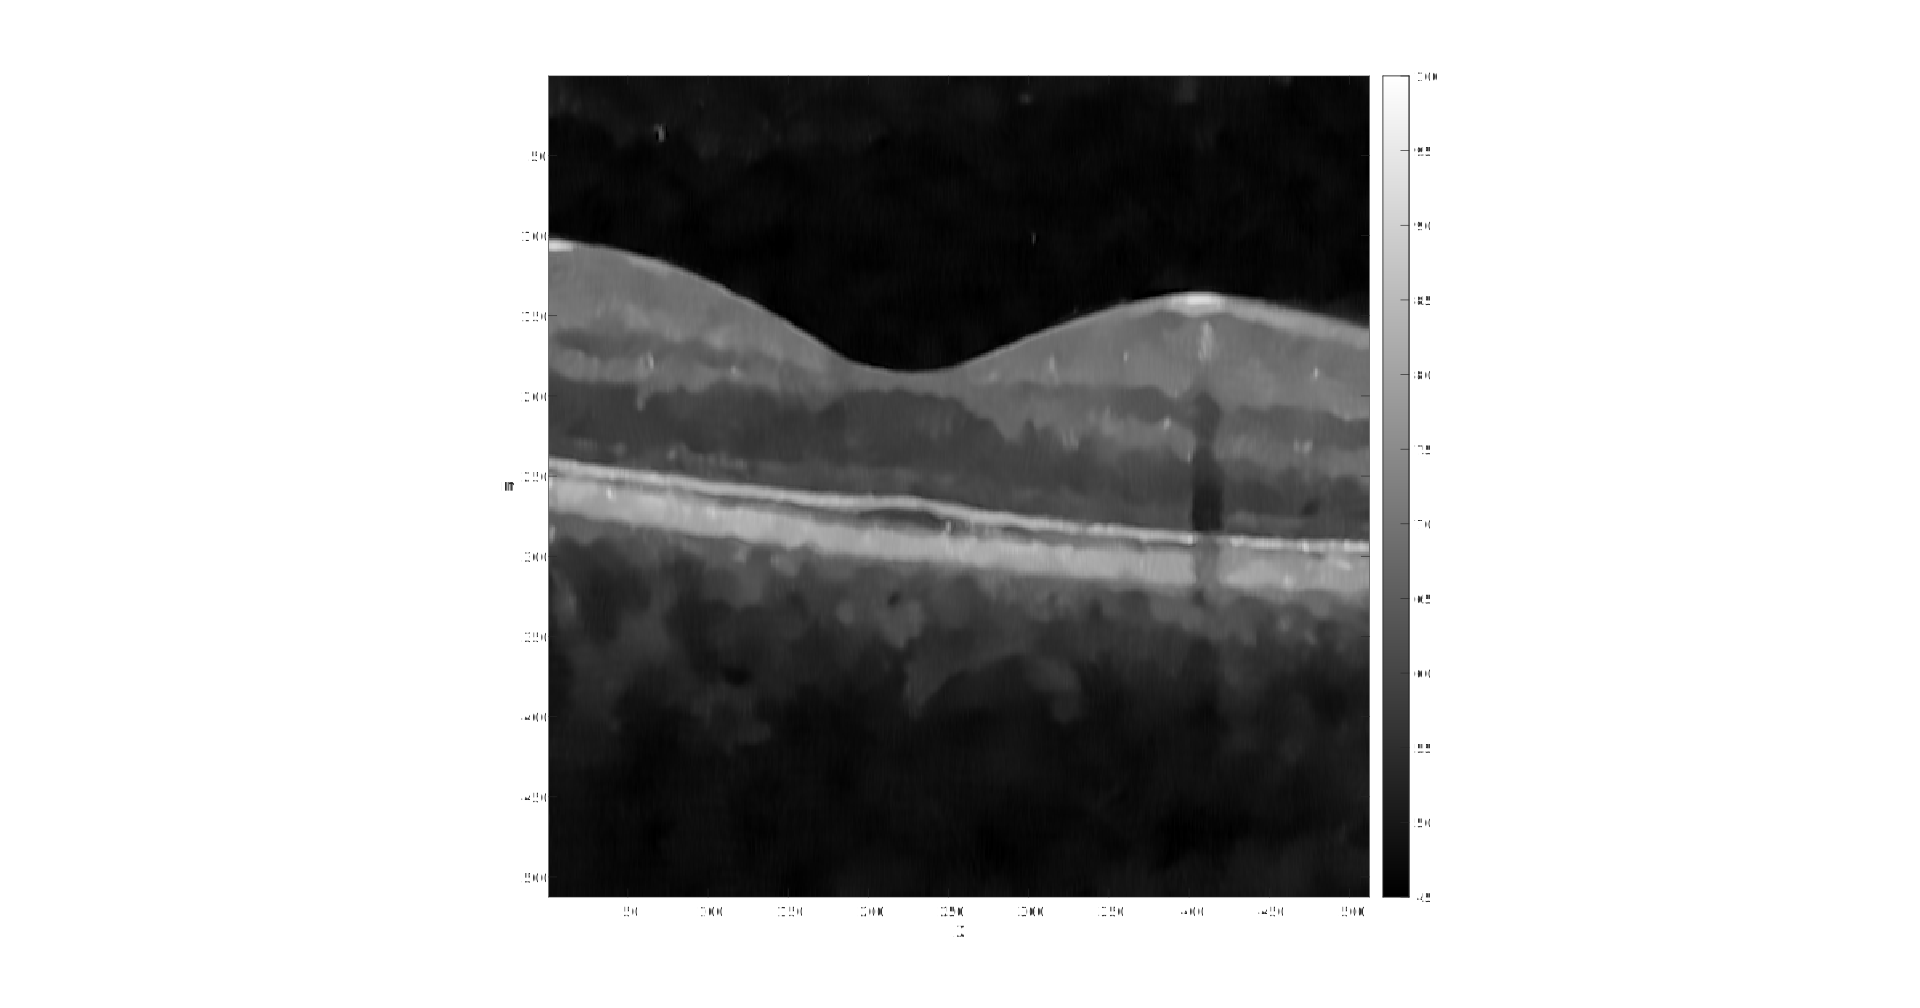
\includegraphics[width=0.49\linewidth]{img/chap3/Retinal_NLMeansIterativo_Bscan128}}
	\subfigure[Filtrado propuesto en ZX.]{\label{subfig:retinal_filtrado_nlmeansOCT_ZX}\includegraphics[width=0.49\linewidth]{img/chap3/Retinal/FinalResult_ZX}}
	\subfigure[Filtado propuesto en ZY.]{\label{subfig:retinal_filtrado_nlmeansOCT_ZY}\includegraphics[width=0.49\linewidth]{img/chap3/Retinal/FinalResult_ZY}}
	\caption[Comparaciones del filtrado propuesto]{Comparación de los resultados obtenidos con \textit{NL-Means}, (a) imagen ruidosa, (b) filtrado con \nlmeans con PPB, (c) filtrado propuesto en dirección $ZX$, y (d) filtrado propuesto en dirección $ZY$.}
	\label{fig:retinal_ima_nlemans_OCT}
\end{figure}

La imagen filtrada con \nlmeansOCT mostrada en la Fig.~\ref{subfig:retinal_filtrado_nlmeansOCT_ZX}, ilustra una mejora en algunos de los problemas mencionados anteriormente en el caso del \nlmeans con PPB, en primer lugar, el efecto \textit{acuarela} ocasionado al filtrar la imagen se ha eliminado completamente. Ésto se le atribuye a dos factores principales, al cubo empleado como ventana de similaridad y al uso de la versión no iterativa del algoritmo. Emplear un cubo como ventana de similaridad tiene la ventaja de que las zonas comparadas aportan información volumétrica de las estructuras en la imagen, por ende, es de esperar que las regiones donde hay transiciones entre capas mantengan su suavidad, ya que a diferencia del \nlmeans con PPB, los cambios de capas no son confundidos con bordes en la imagen al momento de filtrar. Asimismo, emplear el cubo de similaridad aporta información sobre los vecinos cercanos, si éstos siguen la misma distribución de la imagen también ayudarán a realizar el filtrado, previniendo el suavizado excesivo de estructuras finas. De la misma manera, el \speckle que se encuentra en las ventanas de similaridad es volumétrico, por lo tanto el algoritmo identifica más fácilmente la presencia de éste en las ventanas comparadas. Otra ventaja que muestra el resultado filtrado es la conservación de puntos brillantes en la imagen, en general, éstos están asociados con características finas en la imagen, tales como la vasculatura. 

La Fig.~\ref{subfig:retinal_filtrado_nlmeansOCT_ZX} se obtuvo al filtrar el volumen de datos sin corregir el movimiento entre las imágenes que conforman el volumen, por ende, hay desplazamientos aleatorios en el conjunto de datos. Los resultados indican entonces que el filtrado propuesto no depende del desplazamiento axial que puedan tener los datos. Este hecho se explica mediante el cálculo de los pesos, en donde al considerar la similaridad entre las ventanas $\Delta_s$ y $\Delta_t$ no hay una dependencia de la distancia entre ellas, sino que se basa unicamente en la evaluación de la similaridad entre las ventanas. Se espera que independiente del movimiento en los datos el algoritmo escoja aquellos vecinos más parecidos, que aportan la mayor cantidad de información al cálculo de pesos independientemente de su posición respecto a la ventana central, y por lo tanto, al ser completamente \emph{no local}, este algoritmo no se ve muy influenciado por desplazamientos aleatorios en el volumen de datos, siempre que la ventana de búsqueda esté ubicada en la dirección del eje rápido de escaneo, generalmente representada como $ZX$. La corrección del movimiento en los datos, debe producir una mejora en los resultados, pero no es un paso necesario para realizar el filtrado, lo cual es ventajoso en aquellas aplicaciones de OCT en donde la corrección del movimiento es complejo, como en OCT gastrointestinal donde las distorsiones causadas por las contracciones musculares tales como la respiración, y los errores instrumentales como la distorsión rotacional no uniforme (NURD) son complejos de corregir \cite{Liang2016, Uribe2015}. 

Para filtrar los datos con la ventana de búsqueda ubicado en el plano $ZY$, fue necesario la corrección del movimiento axial en lo datos, ya que a diferencia de la dirección $ZX$, la continuidad en la ventana de similaridad $\Delta_s$ se pierde y los vecinos en la ventana de búsqueda pierden la relación, reduciendo la similaridad en la ventana de búsqueda. Además, es importante resaltar que si no se corrige los desplazamientos entre imágenes, los datos son difíciles de interpretar en el plano $ZY$. Luego de corregir el movimiento como lo sugiere Kraus \etal \cite{Kraus2012}, se filtró el volumen con la ventana de búsqueda ubicada sobre $ZY$, y a continuación se realizó la proyección de la imagen de interés, el resultado se presenta en la Fig.~\ref{subfig:retinal_filtrado_nlmeansOCT_ZY}. Con respecto a la corrección de movimiento, se observó la presencia de líneas verticales en la imagen, y una mayor diferenciación de las capas, esto está asociado con que el cubo de similaridad ahora posee una estructura definida en las tres direcciones, lo que incrementa el peso de aquellas zonas similares. No se obtuvo una diferencia significativa al realizar la corrección del movimiento y filtrar sobre el plano $ZX$. %En el caso del plano $ZY$ fue posible filtrar,ya que las ventanas de similaridad contenían estructuras comparables, el resultado obtenido de la proyección en $ZX$ del volumen filtrado en el plano $ZY$ se presenta en Fig.~\ref{subfig:retinal_filtrado_nlmeansOCT_ZY}. La diferencia en las transiciones entre capas está directamente asociada a la corrección del movimiento, aun así, este resultado es comparable a filtrar en dirección $ZX$ y no corregir el desplazamiento, lo que se traduce como una reducción de tiempo de procesamiento, y una ventaja en aquellas aplicaciones donde la corrección de desplazamientos aleatorios no es trivial.

Ahora bien, aunque el filtrado en el plano $ZX$ y $ZY$ parece arrojar resultados similares cuando se realiza la corrección del movimiento, hay implicaciones si se quiere realizan proyecciones sobre planos distintos al de filtrado, como lo muestran la Fig.~\ref{subfig:retinal_filtrado_nlmeansOCT_ZX} y la Fig.~\ref{subfig:retinal_filtrado_nlmeansOCT_ZY}. En el caso de las imágenes \enface del volumen, se obtuvo una diferencia para los diferentes filtrados. La Fig.~\ref{fig:retinal_en_face} muestra la proyección \enface del volumen de datos ruidoso y filtrado en diferentes direcciones. En el caso de los datos ruidosos que se presentan en la Fig.~\ref{subfig:en_face_ima_nsy}, la imagen \enface muestra de manera clara la fóvea en la retina acompañada por algunas venas, sin embargo se percibe la presencia del ruido en la imagen. La Fig.~\ref{subfig:en_face_ima_filt_ZX} es la proyección de los datos luego de realizar el filtrado sobre el plano $ZX$, en este caso se da la aparición de unas \emph{líneas} en la dirección $X$ (verticales), que se encuentran relacionadas con la dirección del filtrado. De la misma manera, al filtrar sobre el plano $ZY$, mostrado en la Fig.~\ref{subfig:en_face_ima_filt_ZY} aparecen una \emph{líneas} ubicadas en la dirección $Y$ (horizontales), estas \emph{líneas} se encuentran relacionadas con el plano de orientación de la ventana de búsqueda. La presencia de las \emph{líneas} sobre la proyección en la dirección del filtrado, sugiere que aunque las imágenes no muestren un efecto evidente de filtrar en distintas direcciones, la proyección \enface va a presentar algunos artefactos en esa dirección. La desventaja del algoritmo se encuentra entonces en que no está bien ajustado para permitir proyecciones diferentes al plano en el cual se lleve a cabo el filtrado. Para comprobar esta hipótesis, se realizó un filtrado tridimensional completo, esto es una ventana de búsqueda tridimensional, así como las ventanas de similaridad en tres dimensiones, con tamaños $W=21\times21\times21$ y $\Delta=7\times7\times7$ respectivamente. El resultado del caso 3D se presenta en la Fig.~\ref{subfig:en_face_ima_filt_3D}, nótese como las \emph{líneas} que se presentaban en la dirección de filtrado se eliminan completamente cuando se realiza el filtro completo en 3D, aun así, la desventaja de este, es un incremento en el tiempo de procesamiento de aproximadamente cinco veces con respecto a \textit{NL-Means-OCT}.


\begin{figure}[ht!]
	\centering
	\subfigure[Datos ruidosos.]{\label{subfig:en_face_ima_nsy}\includegraphics[width=0.2\linewidth]{img/chap3/Retinal/EnfaceNoisy}}
	\subfigure[Filtrado en ZX.]{\label{subfig:en_face_ima_filt_ZX}\includegraphics[width=0.2\linewidth]{img/chap3/Retinal/EnfaceZX}}
	\subfigure[Filtrado en ZY.]{\label{subfig:en_face_ima_filt_ZY}\includegraphics[width=0.2\linewidth]{img/chap3/Retinal/EnfaceZY}}
	\subfigure[Filtrado en 3D.]{\label{subfig:en_face_ima_filt_3D}\includegraphics[width=0.2\linewidth]{img/chap3/Retinal/Enface3D}}
	\caption[Comparación proyecciones \enface filtradas]{Comparación de las proyecciones \enface obtenidas con el volumen de datos. (a) proyección \enface con ruido, (b) proyección luego del filtrado en la dirección $ZX$, (c) imagen \enface obtenida al filtrar en dirección $ZY$ en este caso fue necesaria la corrección del movimiento axial entre las imágenes del volumen de datos, y (d) proyección \enface obtenida con el \nlmeans en 3D.}
	\label{fig:retinal_en_face}
\end{figure}

\subsection{OCT en tractografía}
\label{sec:oct_tractography}

En tractografía, uno de los limitantes que tiene la implementación de técnicas ópticas para la reconstrucción de estructuras y tejidos neuronales, se encuentra en la alta atenuación y esparcimiento que experimenta la luz al interaccionar con este tipo de tejidos. Las técnicas de imagen tradicionales empleadas para tractografía, como la resonancia magnética MRI \cite{Basser2000}, tienen la desventaja de poseer una baja resolución en la reconstrucción, es por esto que han surgido técnicas que permiten el análisis del cerebro a partir de otras formas de generación de imágenes. En ese sentido, Chung \etal \cite{Chung2013} propusieron en el año 2013 una técnica de \emph{blanqueado} para tejidos tales como el cerebro, a esta técnica se le denomina {CLARITY}. En \CLARITY se realiza un proceso de infusión del tejido en monómeros formando una mezcla hidrogel-tejido, luego se da una extracción de lípidos mediante un proceso ionizante, las biomoléculas sin grupo funcional se sacan de la mezcla hidrogel-tejido reduciendo las variaciones en el índice de refracción, y por tanto, disminuyendo el esparcimiento y la absorción por parte del tejido. Esto permite que las estructuras se \textit{aclaren}, siendo posible la penetración de luz hasta un rango de $5-6mm$, lo que permite el uso de la microscopía electrónica para el estudio de las características del cerebro, tales como las sinapsis y las densidades postsinápticas. El problema aquí se encuentra en el tiempo de escaneo, ya que este procedimiento puede tardar varios días, y con la degradación de la muestra y los movimientos que esta pueda sufrir el escaneo puede verse alterado. 

Recientemente, Ku \etal \cite{Ku2016} plantearon un procedimiento adicional a \CLARITY que realiza un escalamiento lineal de las estructuras del cerebro, además de producir el efecto de \emph{blanqueado} necesario para su análisis con técnicas ópticas. El procedimiento de reescalado se realiza mediante la adición de acrilamida a la mezcla de hidrogel-tejido junto con un incremento en la temperatura, así se da una expansión lineal en el tejido, siendo este procedimiento reversible mediante la adición de soluciones salinas. Esta expansión lineal permite el uso de otras técnicas de imagen que pueden lograr escaneos más rápidos y mejores resoluciones, logrando analizar con más detalle estructuras finas al interior de tales tejidos. Ku \etal emplearon microscopía en el límite de difracción para obtener imágenes, sin embargo, otras técnicas como OCT pueden lograr escaneos mucho más rápidos, con tiempos de procesamiento del orden de horas, a cambio de una resolución disminuida. La idea es entonces realizar un escaneo mediante OCT del cerebro de un ratón adulto, considerando las limitantes que tiene OCT, como lo son la disminución en la resolución y la presencia de ruido de \textit{speckle}.

Ahora bien, ligado a este procedimiento de reconstrucción del cerebro por medio de OCT, se encuentra también el proceso de tractografía para obtener un mapa de conexiones (\emph{connectome}) del cerebro \cite{Chang2017} a través del análisis de las sinapsis que éste posee. Para realizar el \emph{connectome} es necesario el cálculo de los gradientes en las tres dimensiones con el volumen de datos, luego se escoge la dirección en la que el gradiente sea menor y esto corresponde a la dirección de las conexiones neuronales que realizan las sinapsis. No obstante, el problema que tiene OCT en este tipo de estudio es la presencia de ruido, particularmente el ruido por \speckle que dificulta altamente la obtención del gradiente, y por ende la reconstrucción de las conexiones, hasta ahora, un estudio de este tipo no ha sido realizado. Es, en este punto, donde \nlmeansOCT es altamente relevante, ya que su capacidad para conservar estructuras finas voluméticras, en este caso las sinapsis, y corregir el ruido de \speckle puede aportar en la reconstrucción del \emph{connectome}. 

A partir de esta información, se realizó el filtrado de un volumen de $160\times3600\times128$ con datos provenientes del escaneo del cerebro de un ratón adulto, el tiempo de procesamiento total fue de $35.4$ horas, y se utilizaron los siguientes parámetros de filtrado: ventana de búsqueda $W=17\times17$, ventana de similaridad $\Delta = 7\times7\times7$ y $h=13$. En la Fig.~\ref{fig:brain} se presenta la sección transversal de las sinapsis (puntos brillantes) para el cerebro del ratón. Para realizar el filtrado, es necesario que esas estructuras brillantes se conserven en sus totalidad, ya que son justamente quienes determinan el mapa de conexiones. La imagen de una región de interés de la sección transversal de las sinapsis obtenida con OCT se presenta en la Fig.~\ref{subfig:brain_ima_nsy_zoom}, mientras que el resultado del filtrado con \nlmeansOCT se muestra en la Fig.~\ref{subfig:brain_ima_filt_zoom}. Las sinapsis aparecen entonces como regiones circulares brillantes, con una alta densidad en la región central de la imagen, y se observan algunas más finas, en tanto que otras son más grandes. Nótese cómo la imagen filtrada elimina la presencia del ruido causado por \speckle y conserva en su totalidad las regiones en donde se hallan las sinapsis. En este caso, se optó por un filtrado más suave comparado con el caso de la retina, ya que aquí las estructuras finas tienen una mayor relevancia, es por ellos que se percibe la presencia de patrones periódicos en la imagen, esto está relacionado con el tamaño del \speckle portador de señal, que es el utilizado para formar imagen. La Fig.~\ref{subfig:brain_ima_nsy} muestra la imagen entera de la sección transversal, y la Fig.~\ref{subfig:brain_ima_filt} la correspondiente filtrada, aquí se evidencia mejor cómo el ruido de la imagen se elimina, mientras se conservan las estructuras finas de la imagen.

La proyección \enface de las sinapsis se presenta en la Fig.~\ref{fig:brain_enface}. La Fig.~\ref{subfig:brain_enface_nsy_zoom} es la proyección a una profundidad que permite observar las sinapsis del cerebro en la región de interés, mientras que la Fig.~\ref{subfig:brain_enface_filt_zoom} es la proyección luego de realizar el filtrado. Éstas imágenes permiten observar cómo el filtrado conserva las sinapsis aun cuando éstas se encuentran superpuestas, y se evidencia cómo conservan forma, estructura y dirección. La Fig.~\ref{subfig:brain_enface_nsy} es la proyección \enface completa de los datos del cerebro y la Fig.~\ref{subfig:brain_enface_filt} es la proyección filtrada.

% \cite{Chung2013,Ku2016,Chang2017}.

\begin{figure}[ht!]
	\centering
	\subfigure[Región de interés en la imagen ruidosa.]{\label{subfig:brain_ima_nsy_zoom}\includegraphics[width=0.49\linewidth]{img/chap3/Brain/ima_nsy_short_brain_lines}}
	\subfigure[Región de interés en la imagen filtrada.]{\label{subfig:brain_ima_filt_zoom}\includegraphics[width=0.49\linewidth]{img/chap3/Brain/ima_filt_short_brain_lines}}
	\subfigure[Imagen ruidosa.]{\label{subfig:brain_ima_nsy}\includegraphics[width=1\linewidth]{img/chap3/Brain/ima_Nsy_brain_lines}}
	\subfigure[Imagen filtrada.]{\label{subfig:brain_ima_filt}\includegraphics[width=1\linewidth]{img/chap3/Brain/ima_filt_brain_lines}}
	\caption[Sección transversal del cerebro de ratón]{Imágenes de la sección transversal del escaneo con OCT de un cerebro de ratón.}
	\label{fig:brain}
\end{figure}

Dadas las características de las ventanas de similaridad tridimensionales, \nlmeansOCT permite realizar el filtrado de estructuras finas en los datos que serán empleados para realizar el \emph{connectome} a partir de las sinapsis en el cerebro. Se espera que este resultado facilite el cálculo del gradiente, y por tanto, mejore la precisión del mapa de conexiones generado, asimismo, facilite la implementación de OCT no solo en tractografía, sino que adicionalmente, en la reconstrucción de tejidos a partir de técnicas de expansión y aclarado, mediante la conservación de las estructuras finas en el volumen de datos.

% images inicial
%\begin{figure}[ht!]
%	\centering
%	\subfigure[Espectro de la fuente.]{\label{subfig:2}\includegraphics[width=0.49\linewidth]{img/chap3/Brain/ima_nsy_short_brain_lines}}
%	\subfigure[Espectro de la fuente con filtro.]{\label{subfig:1}\includegraphics[width=0.49\linewidth]{img/chap3/Brain/ima_filt_short_brain_lines}}
%	\caption{Espectros de la fuente halógena de tungsteno, en (a) la resolución axial es de $0.72\mu m$, mientras que en (b) corresponde a $2.14\mu m$.}
%	\label{fig:2}
%\end{figure}
%
%\begin{figure}[ht!]
%	\centering
%	\subfigure[Espectro de la fuente.]{\label{subfig:2}\includegraphics[width=1\linewidth]{img/chap3/Brain/ima_Nsy_brain_lines}}
%	\subfigure[Espectro de la fuente con filtro.]{\label{subfig:1}\includegraphics[width=1\linewidth]{img/chap3/Brain/ima_filt_brain_lines}}
%	\caption{Espectros de la fuente halógena de tungsteno, en (a) la resolución axial es de $0.72\mu m$, mientras que en (b) corresponde a $2.14\mu m$.}
%	\label{fig:2}
%\end{figure}

\begin{figure}[ht!]
	\centering
	\subfigure[Región de la proyección \enface ruidosa.]{\label{subfig:brain_enface_nsy_zoom}\includegraphics[width=0.49\linewidth]{img/chap3/Brain/Enface_zoomed_nsy_lines}}
	\subfigure[Región de la proyección \enface filtrada.]{\label{subfig:brain_enface_filt_zoom}\includegraphics[width=0.49\linewidth]{img/chap3/Brain/Enface_zoomed_filt_lines}}
	\subfigure[Proyección \enface ruidosa.]{\label{subfig:brain_enface_nsy}\includegraphics[width=1\linewidth]{img/chap3/Brain/Enface_nsy_brain_lines}}
	\subfigure[Proyección \enface filtrada.]{\label{subfig:brain_enface_filt}\includegraphics[width=1\linewidth]{img/chap3/Brain/Enface_filt_brain_lines}}
	\caption[Proyecciones \enface del cerebro del ratón]{Proyecciones \enface con los datos del cerebro del ratón.}
	\label{fig:brain_enface}
\end{figure}

\subsection{OCT gastrointestinal}

En el caso de OCT en tractografía se aprovechó el hecho de que \nlmeansOCT preserva estructuras finas por sus ventanas de similaridad cúbicas. En OCT en gastroenterología, el problema que sufren los datos está relacionado con movimientos aleatorios producidos por fuentes externas al sistema óptico, tales como las contracciones musculares durante la respiración, o el palpito del corazón. Esta vez se pretende aprovechar las características \emph{no locales} del algoritmo, particularmente, porque cómo se observó en la retina, no hay una dependencia entre el filtrado y el movimiento aleatorio en los datos. Particularmente en gastroenterología, los desplazamientos que posean los datos son difíciles de corregir, ya que su naturaleza es básicamente aleatoria y no es fácil de modelar matemáticamente. Sin embargo, hay pequeñas causas de movimiento en los datos como la distorsión rotacional no uniforme (NURD: \textit{non-uniform rotational distortion}) \cite{Uribe2015} que se debe a la rotación de la fibra óptica en el catéter, aun así, no todos los problemas pueden ser corregidos.

Ahora bien, otra característica diferenciadora que tiene OCT gastrointestinal, es que la resolución en las tres direcciones puede ser bastante diferente, es decir, que mientras en la dirección $Z$ es típicamente de $\approx 7\mu m$, en $X$ de $\approx15\mu m$ y en $y$ de $\approx50\mu m$. Para poder obtener un filtrado satisfactorio en este tipo de datos, fue necesario modificar \nlmeansOCT para trabajar con ventanas de similaridad y de búsqueda anisotrópicas, de forma que permitiese la selección preferencia de aquellas direcciones en donde la resolución es mayor. Con esto, se filtró un volumen de $732\times4096\times150$ con datos provenientes del esófago de un paciente, en este caso, el tiempo de procesamiento total fue de $124.7$ horas, y se emplearon los siguientes parámetros: tamaño de la ventana de búsqueda $W = 13\times17$, tamaño de los cubos de similaridad $\Delta=7\times9\times5$ y parámetro $h=13$. El tamaño de la ventana de búsqueda se escogió de manera tal que se privilegia la dirección $X$, ya que en esta es la mayor dimensión; el tamaño de la ventana de similaridad, por su parte, fue escogido para dar más peso a las direcciones en donde la resolución es mayor. La selección de estos parámetros podría realizarse mejor si se realizara un algoritmo que determine el tamaño de las ventanas de similaridad en función del tamaño del \speckle volumétrico, esto se propone como trabajo futuro.

El resultado del filtrado de los datos provenientes de OCT gastrointestinal se presenta en la Fig.~\ref{fig:gastrointestinal}. La Fig.~\ref{subfig:GI_ima_nsy_zoom} es una región de interés que permite comparar fácilmente el resultado contra la imagen filtrada en la Fig.~\ref{subfig:GI_ima_filt_zoom}. La Fig.~\ref{subfig:GI_ima_nsy} es un escaneo tipo B del esófago entero, mientras que la Fig.~\ref{subfig:GI_ima_filt} es la correspondiente filtrada. Las imágenes filtradas muestran nuevamente cómo el algoritmo preserva aquellas estructuras de interés, aunque se percibe una particularidad en este tipo de datos en la parte inferior de las imágenes. En estos lugares, la imagen pareciera ser borrosa, esto se debe a que esa región se encuentra por fuera de la zona focal del sistema, y por ende, aparecen como una región desenfocada. Además de esto, la presencia de estructuras periódicas que aparece en la imagen filtrada, se debe al tamaño del \speckle con el cual se forma imagen (\speckle portador de señal). Se concluye entonces, que aun con el movimiento que este tipo de aplicaciones puede experimentar, \nlmeansOCT puede realizar un filtrado que es independiente de los desplazamientos aleatorios que haya entre los datos, ya que finalmente, lo que se busca son aquellas ventanas de similaridad cuya distribución sea similar para realizar el filtrado.


\begin{figure}[ht!]
	\centering
	\subfigure[Imagen ruidosa en una región de interés.]{\label{subfig:GI_ima_nsy_zoom}\includegraphics[width=0.49\linewidth]{img/chap3/GI/ima_nsy_short_GI_lines}}
	\subfigure[Imagen filtrada en un región de interés.]{\label{subfig:GI_ima_filt_zoom}\includegraphics[width=0.49\linewidth]{img/chap3/GI/ima_filt_short_GI_liens}}
	\subfigure[Imagen ruidosa.]{\label{subfig:GI_ima_nsy}\includegraphics[width=1\linewidth]{img/chap3/GI/ima_nsy_GI_lines}}
	\subfigure[Imagen filtrada.]{\label{subfig:GI_ima_filt}\includegraphics[width=1\linewidth]{img/chap3/GI/ima_filt_GI_lines}}
	\caption[Imágenes del esófago filtradas]{Imágenes filtradas en el caso de datos provenientes de un sistema de OCT gastrointestinal.}
	\label{fig:gastrointestinal}
\end{figure}

Las pruebas realizadas con ventanas de búsqueda cuyo tamaño en una dirección era mucho más grande que en la otra, mostraron la presencia de \textit{línea} en la dirección preferencial, esto es \textit{líneas} verticales en el caso de que $Z>>X$, o \textit{líneas} horizontales cuando $X>>Z$, similares a las comparadas en la proyección \enface para los datos de la retina (Sección~\ref{subsec:oct_retinal}).

\bibliographystyle{unsrt}
\bibliography{ref/Ref_chap_3}